\documentclass[a4paper, 12pt]{article}
\usepackage[T1]{fontenc}
\usepackage{lmodern}
\usepackage{color}
\usepackage{amsfonts}
\usepackage{epstopdf}
\usepackage{matlab}
%\documentclass{book}
\usepackage{blindtext}
\usepackage{hyperref}
\usepackage[brazil]{babel}
\usepackage{amssymb}
\usepackage[utf8]{inputenc}
\usepackage{amsmath}
\usepackage{indentfirst}
\usepackage{graphicx}
\usepackage{multicol,lipsum}
\usepackage[a4paper,
top=3cm, left=3cm, bottom=3cm, right=3cm]{geometry}
\usepackage{setspace}
\usepackage{multirow}
\usepackage{float}
\usepackage[dvipsnames]{xcolor}
\usepackage[table]{xcolor}
%\usepackage{pdflscape}
\usepackage[DIV=15]{typearea}
\usepackage[nottoc]{tocbibind}
\usepackage[sort,numbers]{natbib}
%\usepackage{cite}
\usepackage{matlab}

\usepackage[utf8]{inputenc}
\usepackage[T1]{fontenc}
\usepackage{lmodern}
\usepackage{graphicx}
\usepackage{color}
\usepackage{hyperref}
\usepackage{amsmath}
\usepackage{amsfonts}
\usepackage{epstopdf}
\usepackage[table]{xcolor}
\usepackage{matlab}


\documentclass[letterpaper]{article}
% bib pack %%%%%%%%%%%%%%%%%%%%%%%%%%%%%%%%%%%%%%%%%%%%%%%%%%%%%%%%%%%%%%%%%%%%%
\usepackage[utf8]{inputenc}
\usepackage{geometry}
    \geometry{left=3cm,right=2cm,top=2cm,bottom=2cm}
%
\usepackage[spanish]{babel}
%
\usepackage[fixlanguage]{babelbib}
    \bibliographystyle{babunsrt}
%
\usepackage{url}

\begin{document}
%\maketitle

\begin{titlepage}
	\begin{center}
		

\vspace{10pt}
%\begin{figure}[H][!ht]
%\centering
%
\includegraphics{puc-rio-logo.png}

%\end{figure}
\begin{figure}[!ht]
\centering

\includegraphics{images/puc-rio-logo.png}
\end{figure}
\huge{ Otimização: Algoritmos e Aplicações na Engenharia}
        \vspace{70pt}
        
		\textbf{MEC2403}
		\textbf{\large{\\ }}
		
		\vspace{30pt}
		\textbf{\small{\\Trabalho 02}}
		\vspace{75pt}
		
	\end{center}
	
	\begin{flushleft}
		\begin{tabbing}
			Aluno(a)\qquad\qquad\=\>Paloma Fernanda Loureiro Sette - 1621595\\
			
			Professor(a)\>Ivan Menezes\\
	\end{tabbing}
		  
	\end{flushleft}
	\begin{center}
		%\vspace{\fill}
		\vspace{215pt}
		Rio de Janeiro, 27  de Novembro de 2024
	\end{center}
\end{titlepage}
%%%%%%%%%%%%%%%%%%%%%%%%%%%%%%%%%%%%%%%%%%%%%%%%%%%%%%%%%%%
\newpage
\tableofcontents
\thispagestyle{empty}

\newpage
\pagenumbering{arabic}

\newpage

%\newcommand{\listequationsname}{Lista de Equações}
%\newlistof{myequations}{equ}{\listequationsname}
%\newcommand{\myequations}[1]{%
%\addcontentsline{equ}{myequations}{\protect\numberline{\theequation}#1}\par}

%\listofmyequations
\newpage


\newpage

\listoffigures
\thispagestyle{empty}

\newpage
%%%%%%%%%%%%%%%%%%%%%%%%%%%%%%%%%%%%%%%%%%%%%%%%%%%%%%%%%
%%%%%%%%%%%%%%%%%%%%%%%%%%%%%%%%%%%%%%%%%%%%%%%%%%%

\newpage

\thispagestyle{empty}

\newpage

\section{Introdução}
Este trabalho visa explorar métodos de otimização aplicados à engenharia, em especial as técnicas indiretas de penalidade e de barreira, as quais são amplamente utilizadas na resolução de problemas de otimização com restrições. Tais métodos, que constituem abordagens fundamentais dentro do campo da programação matemática, buscam contornar as restrições de um problema ao transformá-las em termos adicionais na função objetivo, seja para penalizar ou para criar uma barreira que impede a violação das condições impostas. Para isso, será necessário utilizar uma série de algoritmos previamente implementados, como os métodos Univariante, Powell, Steepest Descent, Fletcher–Reeves, BFGS e Newton–Raphson, para a otimização sem restrições. Estes algoritmos serão aplicados aos problemas especificados, utilizando parâmetros e condições iniciais conforme instruído, com o objetivo de encontrar o ponto de mínimo que satisfaça as restrições estabelecidas. A análise dos resultados incluirá também a eficiência de cada método quanto ao número de iterações, convergência e tempo de execução, aspectos que serão devidamente avaliados e este desafio consiste na implementação dos algoritmos de otimização irrestrita para utilização em funções de duas variáveis e em um sistema mecânico, onde deveremos minimizar a Energia Potencial Total para estudos de convergência e demais análises.

\newpage
\section{Objetivos}
O principal objetivo deste trabalho é implementar e analisar a aplicação dos métodos de penalidade e de barreira na resolução de problemas de otimização com restrições. Busca-se, por meio dos experimentos propostos, compreender o comportamento e a eficácia de tais métodos em diferentes cenários, considerando variações nas condições iniciais, parâmetros de penalidade e barreira, além de tolerâncias de convergência. Especificamente, os objetivos incluem:

\begin{enumerate}
    \item Desenvolver algoritmos que incorporem métodos indiretos de penalidade e de barreira para problemas de otimização restrita, utilizando ferramentas de otimização já implementadas para problemas sem restrições;
    \item Avaliar a eficiência e eficácia dos métodos, comparando o número de iterações, o ponto de mínimo obtido, e o tempo de execução de cada abordagem;
    \item Analisar o desempenho dos métodos em relação à precisão e estabilidade frente a problemas com diferentes tipos de restrições, investigando o impacto de variações nos parâmetros de penalidade e barreira sobre a convergência;
    \item Documentar as observações e resultados obtidos para cada método e problema, apresentando gráficos e tabelas que ilustrem o comportamento das funções objetivo e restrições ao longo das iterações.
\end{enumerate}

Esses objetivos visam não apenas a solução dos problemas propostos, mas também a compreensão aprofundada dos métodos de penalidade e barreira no contexto de otimização restrita, contribuindo para a formação de uma base sólida de conhecimento em algoritmos de otimização aplicáveis a problemas práticos de engenharia.


\section{Descrição}

Implementar, usando o MATLAB, os métodos indiretos de \textbf{penalidade} e de \textbf{barreira}. Para a sequência de otimização sem restrições, utilizar os métodos implementados no Trabalho 1, que são:

\begin{enumerate}
\item \textbf{Univariante}
\item \textbf{Powell}
\item \textbf{Steepest Descent}
\item \textbf{Fletcher–Reeves}
\item \textbf{BFGS}
\item \textbf{Newton–Raphson}
\end{enumerate}

Devemos adotar o método da Seção Áurea para a realização das buscas unidirecionais (line search). Para verificação da convergência numérica, utilizar uma tolerância de $10^{-6}$. Em seguida, testar as implementações resolvendo os problemas propostos nos próximos tópicos.



\section{Métodos de Otimização}

\subsection{Otimização com restrições}
Os métodos de penalidade são procedimentos de otimização para problemas com restrições, que transformam um problema com restrições em um problema de minimização sem restrições. Esta transformação é feita adicionando à função objetivo uma parcela que estabelece uma penalidade baseada nas violações das restrições do problema. Dependendo da escolha dos parâmetros de entrada, a função penalizada pode se tornar mal condicionada, tanto numericamente quanto computacionalmente. A expressão abaixo representa a forma geral da pseudo função objetivo:

\begin{equation}
    \Phi(\tilde{x}, r) = f(\tilde{x}) + r \cdot p(\tilde{x})
\end{equation}

Onde: 

$\Phi \rightarrow$ pseudo função objetivo; \\

$\tilde{x} \rightarrow$ variáveis de projeto; \\

$r \rightarrow$ parâmetro de penalidade; \\ 

$p \rightarrow$ função de penalidade; \\ 

\subsubsection{Método da penalidade}

Neste método (também conhecido como "Penalidade Exterior"), a função objetivo é penalizada quando o ponto está fora da região viável. A função $p(\tilde{x})$ é dada por:

\begin{equation}\label{exp_penalidade}
    p(x) = \sum\limits_{i=1}^{m} \left( \max [ 0 , C_i(x)] \right)^2 + \sum\limits_{j=1}^{n} \left[ h_j(x) \right]^2
\end{equation}

Se todas as restrições são satisfeitas, ou seja, nenhuma foi violada, então $p(x) = 0$. Neste caso, a pseudo função objetivo $\Phi(\tilde{x}, r)$ será equivalente à função objetivo original. Caso contrário, a restrição violada será penalizada de acordo com a expressão \eqref{exp_penalidade}. 

O algoritmo que corresponde ao Método de Penalidade pode ser escrito como:

\begin{itemize}
    \item Entrar com os valores iniciais de $\tilde{x}_0$, $r_0$, e $\beta$;
    \item Inicializar contador $k=0$;
    \item Determinar os valores de $\tilde{x}_{k+1}$ que minimizam a pseudo função objetivo $\Phi(\tilde{x}, r_k) = f(\tilde{x}) +\frac{1}{2} r_k p(\tilde{x})$ utilizando um método de otimização sem restrições;
    \item Se $\left| \frac{1}{2} r_k p(\tilde{x}_{k+1}) \right| <$ tolerância, então FIM;
    \item Atualizar $r_{k+1} = \beta \cdot r_k; \quad k = k+1$; retornar ao passo 3.
\end{itemize}

\subsubsection{Método da Barreira}

Neste método, conhecido também como "Penalidade Interior", a função objetivo é penalizada dentro da região viável, de forma que a penalidade aumenta à medida que o ponto $\tilde{x}$ se aproxima da fronteira da região viável. A função $p(\tilde{x})$ é dada por:

\begin{equation}
    p(x) = \sum\limits_{i=1}^{m} - \frac{1}{C_i(x)}
\end{equation}

Ou, usando uma alternativa logarítmica:

\begin{equation}
    p(x) = \sum\limits_{i=1}^{m} \log \left( -C_i(x) \right)
\end{equation}

Vale lembrar que, para o método de barreira, utilizamos apenas restrições de desigualdade $C_i(x) < 0$. Quando houver restrições de igualdade, a pseudo função objetivo ficará na forma:

\begin{equation}\label{exp_barreira}
    \Phi(\tilde{x}, r_k) = f(\tilde{x}) +\frac{1}{2} r_p \sum\limits_{j=1}^{n} \left[ h_j(x) \right]^2 + r_b \sum\limits_{i=1}^{m} - \frac{1}{C_i(x)}
\end{equation}

O algoritmo que corresponde ao Método de Barreira pode ser escrito como:

\begin{itemize}
    \item Entrar com os valores iniciais de $\tilde{x}_0$, $r_0$, e $\beta$;
    \item Inicializar contador $k=0$;
    \item Determinar os valores de $\tilde{x}_{k+1}$ que minimizam a pseudo função objetivo $\Phi(\tilde{x}, r_k) = f(\tilde{x}) + r_b p(\tilde{x})$ utilizando um método de otimização sem restrições;
    \item Se $\left| r_b p(\tilde{x}_{k+1}) \right| <$ tolerância, então FIM;
    \item Atualizar $r_{k+1} = \beta \cdot r_k; \quad k = k+1$; retornar ao passo 3.
\end{itemize}



\subsection{Otimização Sem Restrições}

Como sabemos, métodos de Otimização Sem Restrições (OSR) são técnicas usadas para encontrar o valor mínimo ou máximo de uma função objetivo quando não existem restrições explícitas sobre as variáveis do problema. Em outras palavras, esses métodos assumem que as variáveis podem assumir qualquer valor dentro de um domínio contínuo ou discreto, sem que seja necessário satisfazer restrições ou condições adicionais, como desigualdades ou equações de restrição.\\

Esses métodos se concentram exclusivamente na função objetivo e visam encontrar o ponto onde essa função atinge o mínimo (ou máximo) possível. São amplamente utilizados em problemas onde o domínio de pesquisa é "livre" e onde o objetivo é a otimização pura sem barreiras que limitam o espaço de busca.\\

Os métodos estudados são ponderados nos subtópicos a seguir.

\subsubsection{Método Univariante}

O método Univariante é um dos métodos mais simples de otimização de funções não lineares. Ele opera de forma cíclica, buscando minimização ou maximização ao longo de uma direção de cada vez. Este método realiza uma busca unidimensional em cada iteração, ao longo de cada uma das coordenadas do espaço, alternadamente, até que a convergência seja alcançada. Para ilustrar a ideia do método, consideremos a representação \footnote{Material retirado da Aula 2 do curso "ENG1786 & MEC2403: Otimização: Algoritmos e Aplicações na Engenharia Mecânica", ministrado por Ivan Menezes, PUC-Rio, 27 de agosto de 2024.} esquemática da direção de busca:

\begin{figure}[H]
    \centering
    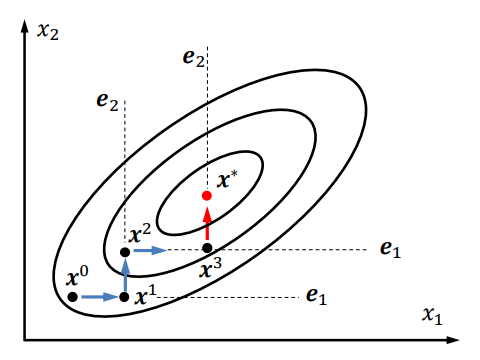
\includegraphics[width=0.6\textwidth]{images/univariante_esquematico.png}
    \caption{Representação da direção de busca do Método Univariante.}
    \label{fig:direction_search_univariate}
\end{figure}

A direção de busca no método univariante é dada pelas direções dos vetores canônicos. Para cada iteração, a busca ocorre ao longo de uma única variável, enquanto todas as outras permanecem constantes. Assim, o vetor de direção $\mathbf{d}^k$ para a $k$-ésima iteração é representado por:

\begin{equation*}
    \mathbf{d}^k = \mathbf{e}_k, \quad k = 1, 2, \dots, n,
\end{equation*}

onde $\mathbf{e}_k$ é o vetor canônico da base:

\begin{equation*}
    \mathbf{e}_k = \{ 0, 0, \dots, 1, \dots, 0, 0 \}^t,
\end{equation*}

em que o valor $1$ está na $k$-ésima posição. A cada iteração, o método realiza uma busca ao longo da direção $\mathbf{e}_k$ e atualiza a posição atual $x^{k+1}$ em direção ao mínimo ao longo dessa coordenada, como ilustrado na Figura \ref{fig:direction_search_univariate}.\\

\textbf{Estratégia de Atualização:} 

\begin{itemize}
    \item Primeiro, seleciona-se a direção de busca $\mathbf{d}^k = \mathbf{e}_k$.
    \item Realiza-se uma busca unidimensional ao longo da direção especificada, utilizando, por exemplo, a Seção Áurea para determinar o valor ótimo de deslocamento.
    \item O ponto é então atualizado de acordo com a equação:

    \begin{equation*}
        x^{k+1} = x^k + \alpha_k \mathbf{d}^k,
    \end{equation*}

    onde $\alpha_k$ é o valor que minimiza a função objetivo ao longo da direção $\mathbf{d}^k$.
\end{itemize}

Após percorrer todas as direções $\mathbf{e}_k$, o método inicia um novo ciclo de busca, até que a convergência seja alcançada ou o critério de parada seja satisfeito. A observação importante aqui é que, se após percorrer todas as direções não for obtida convergência, um novo ciclo deve ser iniciado, conforme destacado na observação da Figura \ref{fig:direction_search_univariate}.\\

\subsubsection{Método de Powell}

O método de Powell é um método de otimização de ordem zero que visa minimizar uma função sem a necessidade de calcular suas derivadas. Ao contrário do método univariante, que apenas utiliza as direções dos eixos canônicos uma a uma, o método de Powell introduz a ideia de criar novas direções de busca a partir dos deslocamentos realizados, permitindo uma convergência mais rápida.\\

Para ilustrar o funcionamento do método de Powell, podemos considerar uma função de duas variáveis, \(f(x_1, x_2)\) e supor que iniciamos a busca por um ponto mínimo a partir de uma posição inicial \(x^0 = [x_1^0, x_2^0]^t\). A ideia principal é minimizar a função ao longo de um conjunto de direções e, em seguida, criar uma nova direção baseada no deslocamento total do ponto inicial até o ponto final do ciclo.\\

Vamos descrever os principais passos do método de Powell de forma mais detalhada e ilustrativa:\\

1. \textbf{Inicialização das Direções}: Começamos com um conjunto de direções canônicas \(\mathbf{e}_1, \mathbf{e}_2, \dots, \mathbf{e}_n\), que representam os eixos coordenados. Para um problema bidimensional, essas direções são simplesmente:
    \[
    \mathbf{e}_1 = \begin{bmatrix} 1 \\ 0 \end{bmatrix}, \quad \mathbf{e}_2 = \begin{bmatrix} 0 \\ 1 \end{bmatrix}
    \]

2. \textbf{Minimização ao Longo das Direções}: A partir do ponto inicial \(x^0\), realizamos a minimização da função ao longo da primeira direção \(\mathbf{e}_1\), encontrando um novo ponto \(x^1\). Em seguida, minimizamos ao longo da segunda direção \(\mathbf{e}_2\), encontrando um ponto \(x^2\). Isso é análogo ao método univariante, mas o diferencial está na criação da nova direção.

3. \textbf{Criação da Nova Direção}: Após minimizar ao longo de todas as direções iniciais, criamos uma nova direção baseada no deslocamento total realizado. Ou seja, a nova direção é definida como:
    \[
    \mathbf{d} = x^2 - x^0
    \]
    Essa nova direção é, na verdade, o vetor que conecta o ponto inicial \(x^0\) ao ponto final \(x^2\) do ciclo atual. A ideia é que essa direção representa um movimento acumulado, possivelmente apontando diretamente para o ponto mínimo.

4. \textbf{Minimização ao Longo da Nova Direção}: Em seguida, minimizamos a função ao longo dessa nova direção \(\mathbf{d}\), encontrando um novo ponto \(x^{0}_{novo}\). Esse ponto será utilizado como ponto inicial para o próximo ciclo.\\

5. \textbf{Atualização das Direções}: Depois de minimizar ao longo da nova direção, substituímos a direção mais antiga (ou uma das direções canônicas) pela nova direção \(\mathbf{d}\). Dessa forma, garantimos que sempre teremos um conjunto atualizado de direções que não são simplesmente ortogonais, mas que podem apontar para direções mais promissoras.\\

6. \textbf{Repetição do Ciclo}: O processo é repetido até que um critério de convergência seja satisfeito. O critério pode ser uma tolerância predefinida ou um número máximo de iterações.\\\\

\textbf{Exemplo}\\

Considere a função quadrática simples:
\[
    f(x_1, x_2) = (x_1 - 3)^2 + (x_2 - 2)^2
\]
Suponha que comecemos do ponto inicial \(x^0 = [0, 0]^t\). Utilizando o método de Powell:\\

- Primeiro minimizamos ao longo de \(\mathbf{e}_1\), movendo na direção do eixo \(x_1\) até um ponto \(x^1 = [3, 0]^t\).\\
- Em seguida, minimizamos ao longo de \(\mathbf{e}_2\), movendo na direção do eixo \(x_2\), até chegar ao ponto \(x^2 = [3, 2]^t\).\\
- Agora criamos uma nova direção baseada no deslocamento total: \(\mathbf{d} = x^2 - x^0 = [3, 2]^t - [0, 0]^t = [3, 2]^t\).\\
- Finalmente, minimizamos ao longo dessa nova direção \(\mathbf{d}\), o que nos leva diretamente ao ponto mínimo \(x^* = [3, 2]^t\).\\

\textbf{Ilustração do Método}\\

A figura abaixo ilustra o método de Powell para a otimização de uma função quadrática, mostrando as direções de busca sucessivas e o caminho tomado até o ponto de mínimo ótimo $x_{\text{opt}}$. O método de Powell é um método de ordem zero que não requer informações de derivada, sendo especialmente adequado para otimização de funções não suaves.

\begin{figure}[H]
    \centering
    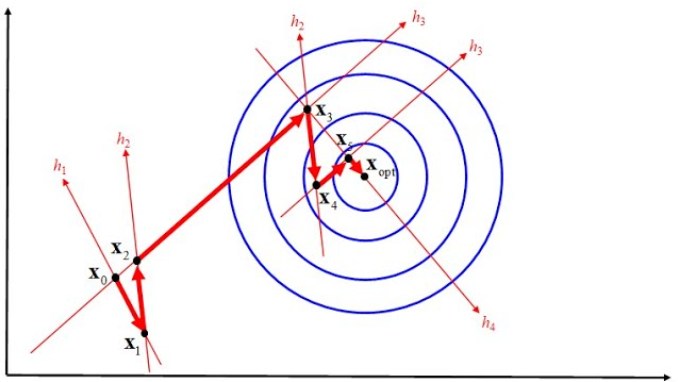
\includegraphics[width=0.65\textwidth]{images/powell_eschematic.png}
    \caption{Ilustração do método de Powell mostrando a progressão até o ponto ótimo $x_{\text{opt}}$. }
    \label{fig:powell_method}
\end{figure}


Na figura, podemos observar:

\begin{itemize}
    \item \textbf{Pontos Iniciais e Intermediários:} O ponto inicial é indicado como $x_0$. A partir deste ponto, o método de Powell faz busca ao longo de uma direção unidimensional, levando ao ponto $x_1$. Este processo se repete ao longo de diferentes direções para encontrar os pontos sucessivos $x_2$, $x_3$ e $x_4$.
    
    \item \textbf{Direções de Busca ($h_1, h_2, h_3, h_4$):} Cada uma das direções $h_k$ representa uma direção de busca ao longo da qual a função é minimizada. O método Powell atualiza dinamicamente essas direções a cada ciclo, utilizando o deslocamento obtido nas iterações anteriores.
    
    \item \textbf{Evolução Até o Mínimo:} As linhas vermelhas representam o caminho seguido até o ponto ótimo $x_{\text{opt}}$. As elipses concéntricas em azul representam as curvas de nível da função objetivo, mostrando como os pontos $x_0, x_1, x_2, x_3, x_4$ se aproximam do ponto ótimo.
    
    \item \textbf{Atualização das Direções:} Após cada ciclo de busca em $n$ direções (correspondente ao número de variáveis), uma nova direção é criada com base no deslocamento acumulado, e o ciclo é repetido até a convergência.
\end{itemize}


\textbf{Nota}: O método de Powell é particularmente eficaz para funções quadráticas e pode gerar direções \(Q\)-conjugadas, o que garante uma convergência mais rápida em comparação aos métodos que utilizam apenas direções ortogonais fixas.

\subsubsection{Método Steepest Descent}

O Método de Steepest Descent (ou Máximo Declive) é um método iterativo utilizado para encontrar o mínimo de uma função diferenciável de várias variáveis. A ideia fundamental do método é mover-se, a partir de um ponto inicial, na direção de maior redução do valor da função objetivo, ou seja, na direção contrária ao gradiente. Assim, o nome "Steepest Descent" surge do fato de o algoritmo sempre seguir a direção em que a função decresce mais rapidamente.\\

Matematicamente, a direção de busca no ponto $x^k$ é dada pelo gradiente da função avaliado nesse ponto, mas apontando na direção oposta:

\begin{equation}
d^k = - \nabla f(x^k)
\end{equation}

O vetor $\nabla f(x^k)$ indica a direção de maior crescimento da função, e ao multiplicarmos por $-1$, obtemos a direção de maior declive da função. Em cada iteração do método, a próxima posição é obtida movendo-se do ponto atual $x^k$ em direção a $d^k$, com um passo de tamanho $\alpha^k$ que pode ser determinado por um procedimento de busca linear:

\begin{equation}
x^{k+1} = x^k + \alpha^k d^k
\end{equation}

O valor de $\alpha^k$ é usualmente escolhido para minimizar a função na direção $d^k$, o que requer uma busca unidimensional para encontrar um ponto onde a função assume um valor mínimo ao longo dessa direção.

O método pode ser descrito de forma algorítmica nos seguintes passos:

\begin{enumerate}
\item Dado um ponto inicial $x^0$, uma tolerância $TOL$ e um número máximo de iterações $MAXITE$, inicializamos $k = 0$.
\item Calculamos a direção de busca como sendo o gradiente negativo da função objetivo no ponto atual:
\begin{equation}
    d^k = -\nabla f(x^k)
\end{equation}
\item Se o valor da norma da direção $||d^k||$ for menor do que a tolerância $TOL$, o processo é encerrado, pois a função já se encontra suficientemente próxima de um ponto estacionário.
\item Caso contrário, determinamos um passo $\alpha^k$ tal que o ponto seguinte minimiza a função na direção $d^k$. Assim, atualizamos a posição para o ponto $x^{k+1}$ conforme:

\begin{equation}
    x^{k+1} = x^k + \alpha^k d^k
\end{equation}
\item Incrementamos $k$ para $k + 1$ e retornamos ao passo 2.
\item Se $k$ atingir $MAXITE$, concluímos que o método não convergiu e paramos.
\end{enumerate}

No contexto visual, o Método de Steepest Descent busca seguir a linha de maior declive a partir do ponto atual, conforme ilustrado na figura a seguir.


\begin{figure}[H]
    \centering
    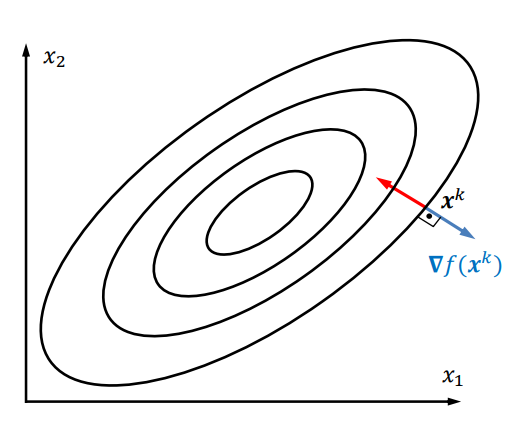
\includegraphics[scale=0.5]{images/steepest.png}
    \caption{Representação gráfica do Método de Steepest Descent}
    
    \label{fig:steepest_descent}
\end{figure}



Nesta figura \footnote{Material retirado da Aula 2 do curso "ENG1786 & MEC2403: Otimização: Algoritmos e Aplicações na Engenharia Mecânica", ministrado por Ivan Menezes, PUC-Rio, 27 de agosto de 2024.}, vemos os contornos de uma função objetivo representados por linhas elípticas, onde cada linha indica um conjunto de pontos de mesmo valor da função. O ponto $x^k$ (marcado em vermelho) é a posição atual do algoritmo, e o vetor $\nabla f(x^k)$ (seta azul) indica a direção de maior aumento da função naquele ponto. A direção de busca utilizada pelo método, \( d^k = -\nabla f(x^k) \), é representada pela seta vermelha, que aponta na direção oposta ao gradiente. Esta é a direção do maior declive, ou seja, a que levará a maior diminuição no valor da função.

Este processo é repetido iterativamente até que o gradiente se aproxime de zero, indicando que o ponto atual está próximo de um ponto estacionário (possível ponto de mínimo).

Esta ilustração facilita a compreensão da dinâmica do método. Imagine que você está tentando descer uma colina: o vetor $\nabla f(x^k)$ aponta a direção de subida mais íngreme, e seguir o vetor oposto, $d^k = -\nabla f(x^k)$, significa descer o mais rápido possível a partir do ponto atual. Ao continuar descendo, o objetivo é se aproximar cada vez mais do ponto de mínimo, que está no centro dos contornos elípticos.

Este método é particularmente útil para problemas em que o cálculo do gradiente é direto e simples. No entanto, apresenta algumas limitações, como a lentidão em funções mal condicionadas, onde as curvas de nível são muito alongadas, fazendo com que o algoritmo siga um caminho "zigue-zague" em direção ao ponto de mínimo. Alternativamente, técnicas como o método de Newton podem superar essas limitações em termos de velocidade de convergência.



\subsubsection{Método de Fletcher-Reeves}

O Método de Fletcher-Reeves é uma variação do método dos Gradientes Conjugados, sendo uma das abordagens mais utilizadas para resolver problemas de otimização sem restrições. Este método é particularmente eficiente para minimizar funções quadráticas, e também pode ser estendido para funções não quadráticas com a utilização de uma busca linear para determinar o tamanho do passo. O método combina elementos dos gradientes descendentes com uma estratégia de busca que permite uma convergência mais rápida, aproveitando as direções conjugadas ao longo das iterações.

O método de Fletcher-Reeves é baseado na premissa de que as direções de busca são tornadas conjugadas em relação à função que está sendo minimizada, resultando em um número menor de iterações necessárias para atingir o mínimo local. 


o método visa resolver problemas de otimização da forma:

\[
\min_x f(x)
\]

onde $f(x)$ é uma função diferenciável que queremos minimizar. A ideia principal do método é iterativamente ajustar a posição atual com uma direção de busca baseada no gradiente, atualizando também um fator de conjugamento, denominado $\beta^k$, que garante que as direções de busca sejam eficientes para atingir o ponto de mínimo de forma otimizada.

O algoritmo pode ser descrito da seguinte forma:\\

1. Inicialize $k = 0$ e um ponto inicial $x^0$.\\
2. Calcule o gradiente $\nabla f(x^0)$. Se $\nabla f(x^0) \approx 0$, a solução foi encontrada e terminamos o algoritmo.\\
3. Caso contrário, defina a direção de busca inicial como $d^0 = -\nabla f(x^0)$.\\
4. Realize uma busca linear para encontrar o tamanho do passo $\alpha^k$, tal que:
   \[
x^{k+1} = x^k + \alpha^k d^k
   \]
5. Atualize o ponto: $x^{k+1} = x^k + \alpha^k d^k$.\\
6. Calcule o novo gradiente $\nabla f(x^{k+1})$.\\
7. Verifique se $\nabla f(x^{k+1}) \approx 0$. Caso positivo, a solução foi encontrada e terminamos o algoritmo.\\
8. Atualize o fator de conjugamento:
   \[
   \beta^k = \frac{(\nabla f(x^{k+1}))^T \nabla f(x^{k+1})}{(\nabla f(x^k))^T \nabla f(x^k)}
   \]
9. Atualize a direção de busca:
   \[
   d^{k+1} = -\nabla f(x^{k+1}) + \beta^k d^k
   \]
10. Aumente o contador de iteração: $k = k + 1$.
11. Retorne ao passo 5.

O valor de $\beta^k$ garante que a nova direção de busca seja conjugada em relação à anterior, tornando a busca mais eficiente. Isso significa que o algoritmo evita revisitar direções já exploradas, proporcionando uma convergência acelerada em comparação ao método do gradiente descendente puro.\\\\

\textbf{- Exemplo de Aplicação:}\\

Vamos aplicar o método a uma função simples para ilustrar os passos. Considere a seguinte função quadrática:

\[
f(x_1, x_2) = x_1^2 + 2x_2^2 - 2x_1x_2 - 4x_1
\]

Queremos encontrar o mínimo dessa função, começando do ponto inicial $x^0 = [2, 1]^t$. Vamos descrever os primeiros passos:

\begin{enumerate}
    \item \textbf{Inicialização}: $x^0 = [2, 1]^t$ e $k = 0$.
    \item \textbf{Cálculo do gradiente}: $\nabla f(x^0) = [2x_1 - 2x_2 - 4, 4x_2 - 2x_1] = [2, 0]$.
    \item \textbf{Direção de busca inicial}: $d^0 = -\nabla f(x^0) = [-2, 0]$.
    \item \textbf{Busca Linear}: Escolhemos um tamanho de passo $\alpha^0$ que minimize $f(x^0 + \alpha d^0)$. Digamos que $\alpha^0 = 0.5$.
    \item \textbf{Atualização do ponto}: $x^1 = x^0 + \alpha^0 d^0 = [1, 1]^t$.
    \item \textbf{Cálculo do novo gradiente}: $\nabla f(x^1) = [0, 0]$. Como o gradiente é zero, atingimos o ponto de mínimo.
\end{enumerate}

Assim, o método de Fletcher-Reeves encontra o mínimo da função em $x^* = [1, 1]^t$.

Este exemplo mostra como o método é eficiente na minimização de funções quadráticas, ajustando iterativamente o ponto de busca com direções conjugadas, garantindo uma convergência mais rápida do que o método do gradiente simples.


\subsubsection{Método BFGS}

O método BFGS (Broyden-Fletcher-Goldfarb-Shanno) é um método de otimização que faz parte dos algoritmos de ordem um, mas com uma aproximação de segunda ordem para obter melhores resultados na minimização de funções. Ele é eficiente porque não necessita calcular a matriz Hessiana explicitamente, mas utiliza informações de primeira ordem (o gradiente) para aproximar a Hessiana e garantir uma boa direção de busca.

O principal objetivo do BFGS é atualizar a matriz $S^k$, que é uma aproximação da inversa da matriz Hessiana, a cada iteração. Dessa forma, é possível melhorar a direção de descida sem precisar calcular a Hessiana diretamente. Isso é feito usando as seguintes fórmulas auxiliares para as variações entre iterações consecutivas:

\begin{equation}
\delta_x^k = x^{k+1} - x^k, \quad \delta_g^k = \nabla f(x^{k+1}) - \nabla f(x^k)
\end{equation}

A atualização da matriz $S^k$ para $S^{k+1}$ é feita por meio da seguinte expressão:

\begin{equation}
S^{k+1} = S^k + \frac{\delta_x^k (\delta_x^k)^T}{(\delta_x^k)^T \delta_g^k} - \frac{S^k \delta_g^k (\delta_g^k)^T S^k}{(\delta_g^k)^T S^k \delta_g^k}
\end{equation}

Essa atualização visa garantir que a nova direção de busca seja uma boa aproximação da direção de descida de Newton, melhorando a eficiência da otimização.\\

\textbf{Passos do Algoritmo BFGS}\\

O método BFGS segue os seguintes passos:

\begin{enumerate}
    \item \textbf{Dados iniciais:} Definimos um ponto inicial $x^0$, uma matriz inicial $S^0 = I$ (matriz identidade), uma tolerância $TOL$ e $k = 0$.
    \item \textbf{Cálculo do gradiente:} Calcula-se o gradiente da função no ponto atual, $\nabla f(x^k)$.
    \item \textbf{Cálculo da direção de busca:} A direção de busca é dada por:
    \begin{equation}
    d^k = - S^k \nabla f(x^k)
    \end{equation}
    \item \textbf{Busca Linear:} Determina-se o tamanho do passo $\alpha^k$ que minimiza a função ao longo da direção de busca $d^k$.
    \item \textbf{Atualização do ponto:} Atualiza-se o ponto atual:
    \begin{equation}
    x^{k+1} = x^k + \alpha^k d^k
    \end{equation}
    \item \textbf{Cálculo do novo gradiente:} Calcula-se $\nabla f(x^{k+1})$.
    \item \textbf{Verificação de convergência:} Se $\|\nabla f(x^{k+1})\| \approx 0$, o algoritmo para e temos o ponto de mínimo. Caso contrário, continua-se.
    \item \textbf{Atualização de $\delta_x^k$ e $\delta_g^k$:}
    \begin{equation}
    \delta_x^k = x^{k+1} - x^k, \quad \delta_g^k = \nabla f(x^{k+1}) - \nabla f(x^k)
    \end{equation}
    \item \textbf{Atualização da matriz $S^k$:} Calcula-se $S^{k+1}$ usando a fórmula de atualização mencionada acima.
    \item \textbf{Incremento do contador:} $k = k + 1$.
    \item \textbf{Repetição:} Voltar ao passo 3.\\
\end{enumerate}

\textbf{Exemplo de Aplicação}\\

Vamos aplicar o método BFGS para minimizar a seguinte função simples:

\begin{equation}
f(x_1, x_2) = x_1^2 + 4x_2^2
\end{equation}

\paragraph{Passo a Passo:}

\begin{itemize}
    \item \textbf{Ponto Inicial:} Vamos escolher o ponto inicial $x^0 = [1, 1]^T$ e a matriz inicial $S^0$ como a matriz identidade:
    \begin{equation}
    S^0 = I = \begin{bmatrix} 1 & 0 \\ 0 & 1 \end{bmatrix}
    \end{equation}
    
    \item \textbf{Cálculo do Gradiente Inicial:} O gradiente da função é dado por:
    \begin{equation}
    \nabla f(x) = \begin{bmatrix} 2x_1 \\ 8x_2 \end{bmatrix}
    \end{equation}
    No ponto inicial $x^0 = [1, 1]^T$:
    \begin{equation}
    \nabla f(x^0) = \begin{bmatrix} 2 \\ 8 \end{bmatrix}
    \end{equation}
    
    \item \textbf{Direção de Busca:}
    \begin{equation}
    d^0 = - S^0 \nabla f(x^0) = - I \begin{bmatrix} 2 \\ 8 \end{bmatrix} = \begin{bmatrix} -2 \\ -8 \end{bmatrix}
    \end{equation}
    
    \item \textbf{Busca Linear:} Suponhamos que a busca linear fornece $\alpha^0 = 0.1$:
    \begin{equation}
    x^1 = x^0 + \alpha^0 d^0 = \begin{bmatrix} 1 \\ 1 \end{bmatrix} + 0.1 \begin{bmatrix} -2 \\ -8 \end{bmatrix} = \begin{bmatrix} 0.8 \\ 0.2 \end{bmatrix}
    \end{equation}
    
    \item \textbf{Cálculo do Novo Gradiente:}
    \begin{equation}
    \nabla f(x^1) = \begin{bmatrix} 2 \times 0.8 \\ 8 \times 0.2 \end{bmatrix} = \begin{bmatrix} 1.6 \\ 1.6 \end{bmatrix}
    \end{equation}
    
    \item \textbf{Atualização de $\delta_x^k$ e $\delta_g^k$:}
    \begin{equation}
    \delta_x^0 = x^1 - x^0 = \begin{bmatrix} 0.8 \\ 0.2 \end{bmatrix} - \begin{bmatrix} 1 \\ 1 \end{bmatrix} = \begin{bmatrix} -0.2 \\ -0.8 \end{bmatrix}
    \end{equation}
    \begin{equation}
    \delta_g^0 = \nabla f(x^1) - \nabla f(x^0) = \begin{bmatrix} 1.6 \\ 1.6 \end{bmatrix} - \begin{bmatrix} 2 \\ 8 \end{bmatrix} = \begin{bmatrix} -0.4 \\ -6.4 \end{bmatrix}
    \end{equation}
    
    \item \textbf{Atualização da Matriz $S^1$:} Com as variações calculadas, aplicamos a fórmula de atualização de $S^k$ para obter $S^1$.
\end{itemize}

O processo é repetido até que a norma do gradiente seja suficientemente pequena, indicando que o ponto de mínimo foi alcançado.\\

O método BFGS é uma ferramenta poderosa para otimização não linear, oferecendo uma convergência eficiente sem a necessidade dos cálculos de segunda ordem exigidos por métodos como Newton. Por meio da atualização iterativa da matriz $S^k$, o método é capaz de ajustar continuamente a direção de busca de uma maneira que acelera a convergência, tornando-o amplamente aplicável em problemas práticos de otimização.

\subsubsection{Método de Newton-Raphson}

O método de Newton-Raphson é uma técnica de otimização que pertence à classe dos métodos de \textbf{ordem dois}. Isso se refere ao uso da matriz \textbf{hessiana}, ou seja, a segunda derivada da função objetivo em relação às variáveis. O método visa encontrar os pontos estacionários da função, ou seja, pontos em que a derivada é zero e, portanto, onde possivelmente temos máximos, mínimos ou pontos de sela.

A ideia central do método é construir uma aproximação linear-quadrática da função, de forma a determinar a direção e o passo que movem a variável de decisão em direção ao mínimo ou máximo desejado. Esse método é amplamente utilizado, pois é mais preciso em encontrar soluções, especialmente quando comparado a métodos de primeira ordem, como o gradiente descendente.

\subsubsection*{Direção de Busca}

No método de Newton-Raphson, a direção de busca $\mathbf{d}^k$ é calculada com base na \textbf{hessiana inversa} $\mathbf{H}(\mathbf{x}^k)^{-1}$ e no \textbf{gradiente} da função $\nabla f(\mathbf{x}^k)$:

\begin{equation}
    \mathbf{d}^k = -\mathbf{H}(\mathbf{x}^k)^{-1} \nabla f(\mathbf{x}^k)
\end{equation}

Neste contexto:
\begin{itemize}
    \item $\mathbf{H}(\mathbf{x}^k)$ é a \textbf{matriz hessiana}, que contém as segundas derivadas parciais da função objetivo, avaliadas no ponto atual $\mathbf{x}^k$. Essa matriz nos dá informações sobre a curvatura da função.
    \item $\nabla f(\mathbf{x}^k)$ é o \textbf{gradiente} da função objetivo, indicando a direção de maior inclinação no ponto atual.
\end{itemize}

\subsubsection*{Explicação Intuitiva}

Para compreender intuitivamente, imagine que estamos tentando encontrar o ponto mais baixo de um vale montanhoso (ou o ponto mais alto, se estivermos maximizando). Se usarmos apenas a inclinação (o gradiente), como no método do gradiente descendente, vamos descer o vale, mas sem levar em consideração a curvatura do terreno — ou seja, não sabemos se estamos descendo uma rampa suave ou caindo de um penhasco.

O método de Newton-Raphson, por outro lado, considera a curvatura do terreno (através da matriz hessiana). Isso significa que ele nos ajuda a prever melhor o "perfil" do vale, ajustando nosso passo de forma mais eficiente, especialmente quando a função possui grandes curvaturas ou mudanças de direção.

\subsubsection*{Demonstração}

Para derivar a fórmula do método de Newton-Raphson, consideramos uma expansão em \textbf{Série de Taylor de segunda ordem} da função $f(\mathbf{x})$, em torno do ponto atual $\mathbf{x}^k$, com um passo $\mathbf{d}^k$:

\begin{equation}
    s(\mathbf{x}) = f(\mathbf{x}^k + \mathbf{d}^k) \approx f(\mathbf{x}^k) + \nabla f(\mathbf{x}^k)^\top \mathbf{d}^k + \frac{1}{2} (\mathbf{d}^k)^\top \mathbf{H}(\mathbf{x}^k) \mathbf{d}^k
\end{equation}

Nosso objetivo é minimizar $s(\mathbf{x})$ em relação ao passo $\mathbf{d}^k$. Portanto, derivamos a expressão acima em relação a $\mathbf{d}^k$ e igualamos a zero:

\begin{equation}
    \frac{d \, s(\mathbf{x})}{d \, \mathbf{d}^k} = 0 \implies \nabla f(\mathbf{x}^k) + \mathbf{H}(\mathbf{x}^k) \mathbf{d}^k = 0
\end{equation}

Reorganizando, obtemos a direção de busca $\mathbf{d}^k$:

\begin{equation}
    \mathbf{d}^k = -\mathbf{H}(\mathbf{x}^k)^{-1} \nabla f(\mathbf{x}^k)
\end{equation}

Assim, podemos ver que a direção $\mathbf{d}^k$ é obtida resolvendo um sistema linear envolvendo a hessiana e o gradiente.

\subsubsection*{Exemplo Simples}

Vamos aplicar o método de Newton-Raphson a uma função quadrática simples:

\begin{equation}
    f(x) = x^2 - 4x + 4
\end{equation}

Primeiro, encontramos o gradiente e a hessiana:
\begin{itemize}
    \item \textbf{Gradiente}: $\nabla f(x) = 2x - 4$
    \item \textbf{Hessiana}: $\mathbf{H} = 2$
\end{itemize}

No ponto inicial $x^0 = 0$:
\begin{itemize}
    \item $\nabla f(0) = -4$
    \item $\mathbf{H} = 2$
\end{itemize}

Calculando a direção de busca:

\begin{equation}
    d^0 = -\mathbf{H}^{-1} \nabla f(0) = -\frac{1}{2} \cdot (-4) = 2
\end{equation}

Assim, o próximo ponto é:

\begin{equation}
    x^1 = x^0 + d^0 = 0 + 2 = 2
\end{equation}

No ponto $x = 2$, podemos verificar que o gradiente é zero, indicando que chegamos a um ponto crítico (neste caso, um mínimo).

\subsubsection*{Observações}

\begin{itemize}
    \item O método de Newton-Raphson \textbf{converge muito rapidamente} para um mínimo quando a aproximação inicial está "perto" da solução exata, graças ao uso da informação da curvatura.
    \item No entanto, o método pode falhar se a hessiana não for positiva definida ou se estivermos longe do mínimo, pois a inversão da hessiana se torna instável.
\end{itemize}






\newpage
\section{Primeiro Problema}
\begin{equation}
     p(t) = \left\{ \begin{array}{rcl}
            Min \>\ f(x_1, x_2) = (x_1 - 2)^2 + (x_2 - 2)^2 \\ \\
            s.t.: \>\ x_1 + x_2 + 3 \leq 0           \end{array} \right.
\end{equation} \\

OBS.: Adotar $r_p ^0=0.1$, $\beta = 10$ e $x^0 = \{-5,-2\}$ para o método de penalidade e $r_b ^0=10$, $\beta = 0.1$ e $x^0 = \{-5,-2\}$ para o método de barreira. \\

\subsection{Entendendo o Problema}

%% Relação entre Otimização Sem Restrições (OSR) e Otimização Com Restrições (OCR)

A questão proposta envolve um problema de otimização com restrições (OCR), especificando a necessidade de aplicação de métodos indiretos de \textbf{penalidade} e \textbf{barreira} para resolvê-lo. O enunciado sugere a utilização dos métodos implementados previamente para otimização sem restrições (OSR) – tais como Univariante, Powell, Steepest Descent, Fletcher-Reeves, BFGS e Newton-Raphson – para resolver o problema. Neste contexto, é importante compreender como relacionar OCR e OSR.\\

Os métodos de \textbf{penalidade} e \textbf{barreira} são técnicas que permitem transformar um problema de otimização com restrições em um problema equivalente sem restrições. Essa transformação é alcançada adicionando-se à função objetivo termos que representam as restrições:\\ 

\begin{itemize}
    \item \textbf{Método de Penalidade Exterior}: consiste em adicionar à função objetivo uma penalidade proporcional à violação das restrições. A função objetivo penalizada é dada por:
      
      \begin{equation}
      \phi(\mathbf{x}, r_p) = f(\mathbf{x}) + r_p \cdot \max(0, g(\mathbf{x}))^2
      \end{equation}
      
      onde $g(\mathbf{x}) \leq 0$ representa as restrições do problema. Este método cria um problema sem restrições ao adicionar uma penalidade que cresce com o aumento da violação das restrições. O parâmetro $r_p$ é aumentado iterativamente para garantir que a solução se torne cada vez mais próxima de uma solução viável.

      \item \textbf{Método de Barreira Interior}: consiste em adicionar à função objetivo uma função de barreira que impede a violação das restrições. A função objetivo com barreira é dada por:
      
      \begin{equation}
      \phi(\mathbf{x}, r_b) = f(\mathbf{x}) - \frac{r_b}{g(\mathbf{x})}
      \end{equation}
    
      Este método cria uma barreira que cresce infinitamente quando a solução se aproxima da fronteira da região viável, garantindo que o ponto otimizado permaneça dentro da região permitida pelas restrições.
    
\end{itemize}



Uma vez transformado o problema com restrições em um problema sem restrições, torna-se possível utilizar os \textbf{métodos de Otimização Sem Restrições} (OSR), tais como os implementados no Trabalho 1 (Univariante, Powell, Steepest Descent, Fletcher-Reeves, BFGS e Newton-Raphson), para encontrar o mínimo da pseudo-função objetivo. Assim, a resolução do problema ocorre em duas etapas principais:

\begin{enumerate}
    \item \textbf{Transformação do Problema}: Utiliza-se o método de penalidade ou barreira para converter o problema de OCR em um problema de OSR, criando uma nova função objetivo $\phi(\mathbf{x})$ que incorpora as restrições.
    \item \textbf{Otimização Sem Restrições}: Aplica-se um dos métodos de OSR para minimizar a pseudo-função objetivo $\phi(\mathbf{x})$, obtendo a solução que respeita as restrições originais.

\end{enumerate}

Dessa forma, a relação entre OCR e OSR está justamente na transformação do problema. Ao resolver o problema com restrições por métodos indiretos, transformamos o problema em um equivalente sem restrições e, em seguida, aplicamos as técnicas de otimização previamente desenvolvidas.\\

\subsection{Parâmetros e Configurações do Problema}
Para o método de penalidade, os parâmetros fornecidos incluem um valor inicial de penalidade $r_p^0 = 0.1$, fator de crescimento $\beta = 10$, e ponto inicial $\mathbf{x}^0 = [-5, -2]$. Para o método de barreira, temos um valor inicial de barreira $r_b^0 = 10$, fator de decaimento $\beta = 0.1$, e o mesmo ponto inicial. Estes parâmetros determinam como a penalidade ou barreira serão ajustadas iterativamente, até que a solução atenda às condições de convergência desejadas.

Portanto, a utilização de métodos de OSR como parte do processo de resolução de problemas de OCR é uma abordagem eficaz que facilita o tratamento das restrições, especialmente ao utilizar técnicas bem compreendidas e eficientes para otimização sem restrições.

\subsection{Método de Penalidade}

O Método de Penalidade Exterior transforma o problema original de otimização com restrições em um problema sem restrições, adicionando um termo de penalidade que representa as restrições. Dessa forma, a minimização é conduzida iterativamente sobre uma pseudo-função que incorpora tanto a função objetivo quanto uma penalidade proporcional à violação das restrições. Esta penalidade é ajustada iterativamente através de um parâmetro de penalidade ($r_p$), que é aumentado a cada passo, a fim de assegurar que a solução se torne cada vez mais próxima de uma solução viável que respeite as restrições impostas.

\subsubsection{Resultados dos Métodos OSR Utilizados}

Nesta seção, apresentamos os resultados dos diferentes métodos de Otimização Sem Restrições (OSR) aplicados ao problema transformado pelo Método de Penalidade. Após a implementação e a execução do algoritmo aplicada à função com suas restrições, obtivemos a seguinte saída:

\begin{verbatim}
- MÉTODO UNIVARIANTE:
Mínimo encontrado: [-1.503521, -1.496130]^t
Valor da Função Objetivo: 24.497581
Número de Iterações: 5
Tempo de Execução: 0.968349 segundos
**********************************
- MÉTODO POWELL:
Mínimo encontrado: [-1.978980, -1.020624]^t
Valor da Função Objetivo: 24.956450
Número de Iterações: 5
Tempo de Execução: 0.136063 segundos
**********************************
- MÉTODO STEEPEST DESCENT:
Mínimo encontrado: [-1.917005, -1.917008]^t
Valor da Função Objetivo: 30.685878
Número de Iterações: 5
Tempo de Execução: 0.279750 segundos
**********************************
- MÉTODO FLETCHER-REEVES:
Mínimo encontrado: [-1.499826, -1.499826]^t
Valor da Função Objetivo: 24.497571
Número de Iterações: 5
Tempo de Execução: 2.428321 segundos
**********************************
- MÉTODO NEWTON-RAPHSON:
Mínimo encontrado: [-1.500126, -1.500126]^t
Valor da Função Objetivo: 24.501762
Número de Iterações: 5
Tempo de Execução: 0.253179 segundos
**********************************
- MÉTODO BFGS:
Mínimo encontrado: [-1.499825, -1.499825]^t
Valor da Função Objetivo: 24.497550
Número de Iterações: 5
Tempo de Execução: 0.009265 segundos
**********************************
\end{verbatim}




A tabela \ref{tab:penalidade_results} resume os resultados obtidos no MATLAB, apresentando o ponto mínimo encontrado, o valor da função objetivo, o número de iterações e o tempo de execução de cada método.

\begin{table}[h!]
    \centering
    \resizebox{\textwidth}{!}{
    \begin{tabular}{|l|c|c|c|c|}
        \hline
        \textbf{Método} & \textbf{Mínimo Encontrado} & \textbf{Valor da Função Objetivo} & \textbf{Iterações} & \textbf{Tempo de Execução (s)} \\
        \hline
        Univariante & [-1.503521, -1.496130] & 24.497581 & 5 & 0.968349 \\
        Powell & [-1.978980, -1.020624] & 24.956450 & 5 & 0.136063 \\
        Steepest Descent & [-1.917005, -1.917008] & 30.685878 & 5 & 0.279750 \\
        Fletcher-Reeves & [-1.499826, -1.499826] & 24.497571 & 5 & 2.428321 \\
        Newton-Raphson & [-1.500126, -1.500126] & 24.501762 & 5 & 0.253179 \\
        BFGS & [-1.499825, -1.499825] & 24.497550 & 5 & 0.009265 \\
        \hline
    \end{tabular}
    }
    \caption{Resultados dos Métodos OSR para o Método de Penalidade}
    \label{tab:penalidade_results}
\end{table}


\subsubsection*{Análise dos Resultados}

Os resultados mostram diferenças consideráveis entre os métodos em termos de precisão, número de iterações e tempo de execução:

\begin{itemize}
    \item \textbf{Método Univariante}: O método Univariante apresentou uma solução próxima do ótimo, com um valor da função objetivo de 24.497581 e um ponto mínimo em \([-1.503521, -1.496130]\). Contudo, o tempo de execução (0.968349 s) foi relativamente alto, comparado a outros métodos, indicando uma desvantagem na sua eficiência.
    \item \textbf{Método Powell}: O método de Powell teve um dos melhores desempenhos em termos de tempo de execução (0.136063 s), sendo o segundo mais rápido, embora o valor da função objetivo obtido (24.956450) fosse ligeiramente maior do que o valor ótimo encontrado por outros métodos. Apesar disso, o método é interessante para problemas em que se precisa de soluções rápidas.
    \item \textbf{Método Steepest Descent}: Este método convergiu para um ponto \([-1.917005, -1.917008]\), mas apresentou um valor da função objetivo significativamente maior (30.685878), sugerindo que não conseguiu aproximar-se de uma solução ótima de forma efetiva. A convergência lenta e a precisão limitada indicam que este método não foi o mais adequado para o problema, apesar do tempo de execução razoável (0.279750 s).
    \item \textbf{Método Fletcher-Reeves}: O método de Fletcher-Reeves, que faz parte da classe dos gradientes conjugados, obteve uma solução precisa (\([-1.499826, -1.499826]\)) com valor da função objetivo de 24.497571. No entanto, o tempo de execução foi o maior de todos (2.428321 s), indicando que, embora precise, a abordagem é computacionalmente custosa.
    \item \textbf{Método Newton-Raphson}: Newton-Raphson apresentou resultados bastante próximos do ótimo (\([-1.500126, -1.500126]\)), com valor da função objetivo de 24.501762. O tempo de execução foi relativamente curto (0.253179 s), mostrando um equilíbrio entre eficiência e precisão.
    \item \textbf{Método BFGS}: O método BFGS foi o mais eficaz, tanto em termos de precisão quanto de tempo de execução. Encontrou um ponto próximo do ótimo (\([-1.499825, -1.499825]\)), com valor da função objetivo de 24.497550. O tempo de execução de apenas 0.009265 s destaca a eficiência do método em termos computacionais, tornando-o a escolha mais indicada para o problema.
\end{itemize}


\subsubsection*{Comparação entre os Métodos}

Podemos destacar algumas observações importantes:

\begin{enumerate}
    \item \textbf{Precisão}: Métodos como Univariante, Fletcher-Reeves, Newton-Raphson e BFGS apresentaram valores da função objetivo muito próximos, sugerindo boa precisão na solução. Entre eles, o BFGS apresentou o menor valor de função objetivo, o que indica uma solução próxima do ótimo global.
    \item \textbf{Eficiência}: O método BFGS se destacou por ser muito mais eficiente em termos de tempo de execução, enquanto métodos como Fletcher-Reeves, embora precisos, foram computacionalmente mais custosos.
    \item \textbf{Limitações do Steepest Descent}: O método de Steepest Descent apresentou a menor qualidade de solução, não conseguindo convergir para um valor próximo do ótimo. Além disso, seu custo computacional não compensou a baixa precisão, sendo, portanto, o menos eficiente para este problema.
\end{enumerate}

\subsubsection*{Análise da Curva de Nível}

A curva de nível da função objetivo representa as linhas de igual valor para a função \( f(x_1, x_2) = (x_1 - 2)^2 + (x_2 - 2)^2 \). Esses contornos são indicativos de regiões de mesmo valor da função, com as curvas internas indicando valores mais baixos, ou seja, a direção de descida da função. A linha vermelha tracejada mostra a **fronteira da restrição**, que delimita a região viável, determinada pela condição \( x_1 + x_2 + 3 \leq 0 \). Essa região é a área à esquerda da linha, onde as soluções são consideradas viáveis.\\

No gráfico, cada ponto colorido corresponde à solução obtida por um método diferente. Esses pontos representam os valores encontrados após a aplicação dos métodos de Otimização Sem Restrições (OSR) ao problema de Penalidade Exterior.\\

Podemos observar que os pontos ótimos encontrados por diferentes métodos de OSR estão localizados próximos à linha da restrição, sugerindo que os métodos conseguiram, em sua maioria, encontrar valores minimizadores que respeitam a restrição imposta. No entanto, há diferenças sutis nas localizações dos pontos, indicando pequenas variações nos mínimos encontrados. Isso pode ser atribuído à natureza de cada método de OSR e como eles lidam com o problema transformado pela penalidade.\\

Todos os métodos convergiram para uma região próxima da \textbf{fronteira da restrição}, indicando que a transformação realizada pelo método de penalidade foi eficaz em forçar a solução para uma região factível. Vale destacar que o método Steepest Descent parece ter se afastado mais da região dos outros pontos, o que é consistente com sua maior imprecisão no valor da função objetivo.\\

O ponto encontrado pelo \textbf{Método BFGS} (representado pelo marcador preto) está visivelmente mais próximo da solução esperada, conforme indicado pela concentração das curvas de nível mais próximas ao centro. O \textbf{Método Steepest Descent} (marcador verde) está localizado mais afastado das regiões de menor valor, o que evidencia sua dificuldade em se aproximar do ótimo global em relação aos outros métodos.\\

Os métodos \textbf{Univariante}, \textbf{Fletcher-Reeves}, \textbf{Newton-Raphson}, e \textbf{BFGS} encontraram pontos bastante próximos, indicando uma solução semelhante em termos de valor da função objetivo e posição no espaço de busca. Esse agrupamento reforça a conclusão de que esses métodos são mais adequados para este tipo de problema, uma vez que são capazes de encontrar soluções otimizadas de forma consistente.

\paragraph{Comportamento da Penalidade}

O método de penalidade aplicado neste problema faz com que os pontos de minimização sejam empurrados em direção à fronteira da restrição, à medida que o parâmetro de penalidade (\( r_p \)) é aumentado. Essa característica é visível no gráfico, já que todos os pontos se situam muito próximos da linha da restrição. A penalidade utilizada neste método funciona ao elevar o custo da solução quando uma violação da restrição ocorre, tornando a solução fora da região factível indesejável.

\paragraph{Interpretação da Eficiência Visual}

Podemos observar também a trajetória dos métodos ao longo das curvas de nível, sugerindo como cada método avançou em direção ao mínimo. No gráfico, é possível perceber como alguns métodos (como Powell e Newton-Raphson) tenderam a convergir de forma mais direta para a solução, enquanto métodos como o Steepest Descent pareceram mais erráticos, indicando uma menor eficiência em convergir para o ponto ótimo.\\


Portanto, o gráfico de curva de nível fornece uma visão intuitiva da diferença na performance dos métodos. Vemos claramente que, enquanto a maioria dos métodos encontrou soluções aceitáveis, o Método BFGS apresentou a solução mais próxima ao centro das curvas de nível, confirmando sua precisão superior. O Método Steepest Descent, apesar de encontrar um ponto próximo da fronteira, claramente não conseguiu otimizar adequadamente o valor da função objetivo, como indicado pela sua maior distância em relação ao centro das curvas de nível.

Assim, a análise gráfica corrobora as conclusões obtidas a partir dos resultados numéricos: o \textbf{Método BFGS} se destaca como o método mais eficiente e preciso, enquanto \textbf{Steepest Descent} se mostra menos eficaz tanto em termos de convergência quanto de precisão da solução.


\begin{figure}[H]
\centering
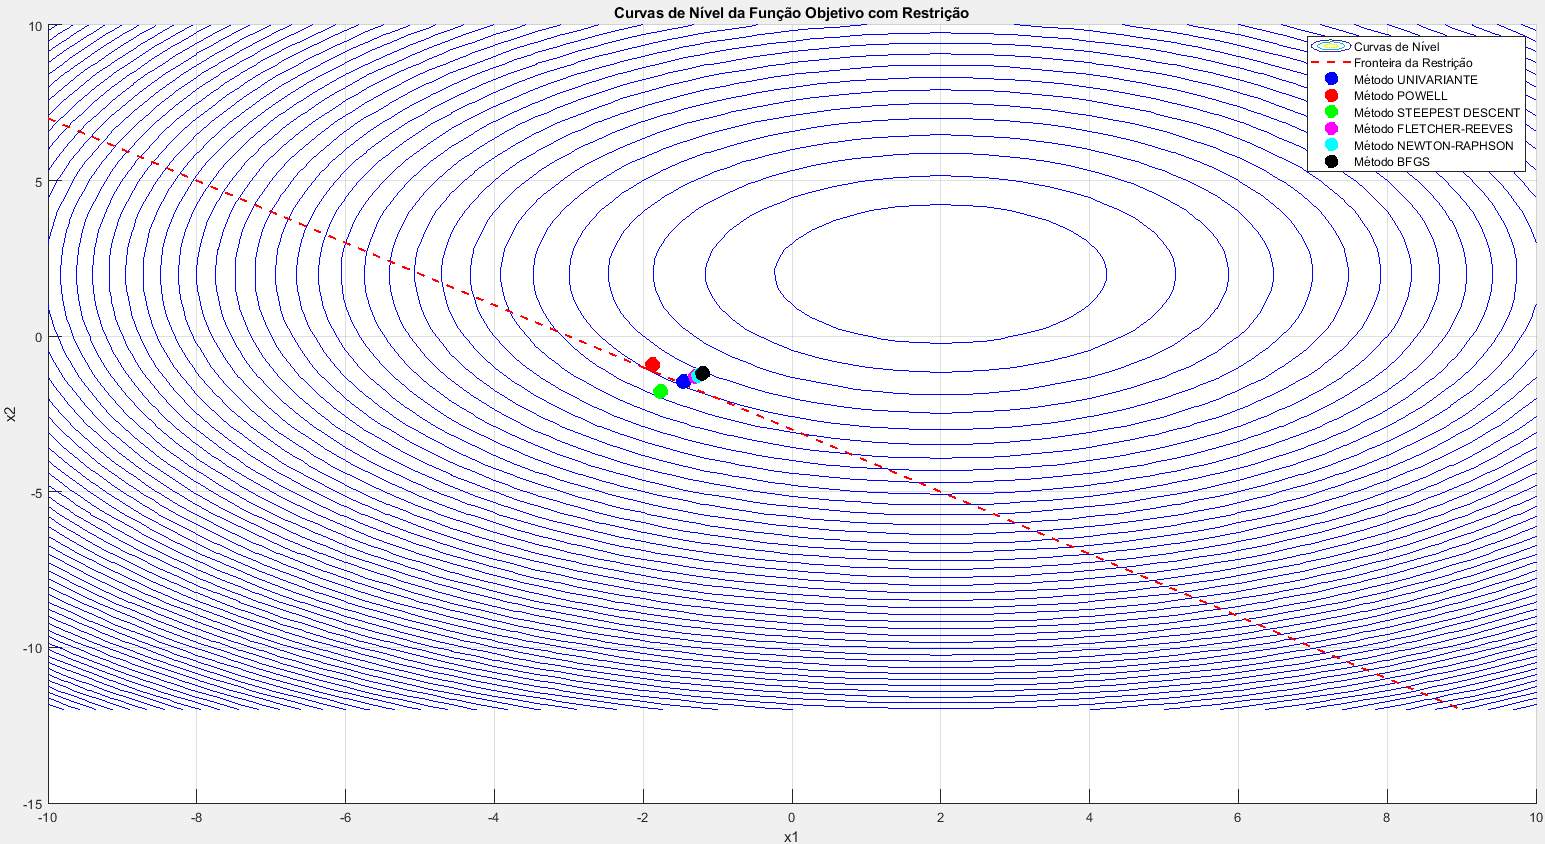
\includegraphics[scale = 0.4]{images/curva_de_nivel_funcao1_penalidade.png}
\label{filtro1}
\caption{Curva de Nível - Função 1: Aplicação do Método da Penalidade}
\end{figure}



Os resultados obtidos indicam que a escolha do método de otimização sem restrições tem impacto direto na eficiência e precisão do Método de Penalidade. Neste estudo, o método BFGS destacou-se como o mais eficiente, com excelente precisão e um tempo de execução extremamente curto. Métodos como Steepest Descent se mostraram ineficazes, enquanto Fletcher-Reeves e Newton-Raphson, embora precisos, apresentaram um custo computacional mais elevado.

Portanto, a combinação do Método de Penalidade com o BFGS foi a mais vantajosa para este problema específico, oferecendo um equilíbrio adequado entre precisão e eficiência computacional.






\newpage
\subsection{Método de Barreira}

O Método de Barreira Interior transforma o problema original de otimização com restrições em um problema sem restrições, adicionando um termo de barreira que impede a violação das restrições. Dessa forma, a minimização é realizada sobre uma pseudo-função que incorpora tanto a função objetivo quanto um termo de barreira que cresce conforme a solução se aproxima da fronteira da região viável. Esse termo impede que a solução ultrapasse as fronteiras impostas pelas restrições.

No Método de Barreira, o termo é ajustado iterativamente através de um parâmetro de barreira ($r_b$), que é diminuído ao longo das iterações, a fim de assegurar que a solução final esteja o mais próxima possível do ótimo dentro da região factível.

\subsubsection{Resultados dos Métodos OSR Utilizados}

Nesta seção, apresentamos os resultados obtidos ao aplicar o Método de Barreira ao problema de otimização com restrições, transformando-o em um problema sem restrições e utilizando diferentes métodos de Otimização Sem Restrições (OSR) para resolver a pseudo-função criada. Os resultados estão apresentados a seguir:

\begin{verbatim}
- MÉTODO UNIVARIANTE:
Mínimo encontrado: [-1.652476, -0.472136]^t
Valor da Função Objetivo: 19.452036
Número de Iterações: 310
Tempo de Execução: 0.036792 segundos
**********************************
- MÉTODO POWELL:
Mínimo encontrado: [-31.935322, 29.875753]^t
Valor da Função Objetivo: 1928.663692
Número de Iterações: 310
Tempo de Execução: 0.039271 segundos
**********************************
- MÉTODO STEEPEST DESCENT:
Mínimo encontrado: [NaN, NaN]^t
Valor da Função Objetivo: NaN
Número de Iterações: 1000
Tempo de Execução: 105.571753 segundos
**********************************
- MÉTODO FLETCHER-REEVES:
Mínimo encontrado: [NaN, NaN]^t
Valor da Função Objetivo: NaN
Número de Iterações: 1000
Tempo de Execução: 26.563223 segundos
**********************************
- MÉTODO NEWTON-RAPHSON:
Mínimo encontrado: [NaN, NaN]^t
Valor da Função Objetivo: NaN
Número de Iterações: 1000
Tempo de Execução: 31.648942 segundos
**********************************
- MÉTODO BFGS:
Mínimo encontrado: [NaN, NaN]^t
Valor da Função Objetivo: NaN
Número de Iterações: 1000
Tempo de Execução: 54.964462 segundos
**********************************
\end{verbatim}

A tabela \ref{tab:barreira_results} resume os resultados obtidos no MATLAB, apresentando o ponto mínimo encontrado, o valor da função objetivo, o número de iterações e o tempo de execução de cada método.

\begin{table}[h!]
    \centering
    \resizebox{\textwidth}{!}{
    \begin{tabular}{|l|c|c|c|c|}
        \hline
        \textbf{Método} & \textbf{Mínimo Encontrado} & \textbf{Valor da Função Objetivo} & \textbf{Iterações} & \textbf{Tempo de Execução (s)} \\
        \hline
        Univariante & [-1.652476, -0.472136] & 19.452036 & 310 & 0.036792 \\
        Powell & [-31.935322, 29.875753] & 1928.663692 & 310 & 0.039271 \\
        Steepest Descent & [NaN, NaN] & NaN & 1000 & 105.571753 \\
        Fletcher-Reeves & [NaN, NaN] & NaN & 1000 & 26.563223 \\
        Newton-Raphson & [NaN, NaN] & NaN & 1000 & 31.648942 \\
        BFGS & [NaN, NaN] & NaN & 1000 & 54.964462 \\
        \hline
    \end{tabular}
    }
    \caption{Resultados dos Métodos OSR para o Método de Barreira}
    \label{tab:barreira_results}
\end{table}

\subsubsection{Análise dos Resultados}

Os resultados obtidos a partir do Método de Barreira mostram um comportamento bastante distinto em relação aos métodos utilizados. O método transformou o problema com restrições em um problema sem restrições, o qual foi resolvido pelos métodos de Otimização Sem Restrições (OSR). No entanto, observamos uma dificuldade significativa para os métodos que dependem do cálculo do gradiente. Abaixo, segue uma análise detalhada de cada método:

\begin{itemize}
    \item \textbf{Método Univariante}: O método Univariante apresentou um resultado viável, encontrando um ponto mínimo em \([-1.652476, -0.472136]\), com valor da função objetivo de 19.452036. O número de iterações foi 310, e o tempo de execução foi relativamente curto (0.036792 s). A convergência ocorreu sem problemas, indicando que o método foi capaz de lidar bem com a transformação da função original.
    
    \item \textbf{Método Powell}: O método de Powell apresentou um comportamento inesperado, com o mínimo encontrado em \([-31.935322, 29.875753]\), resultando em um valor da função objetivo de 1928.663692. O número de iterações foi o mesmo do método Univariante (310), mas o valor encontrado sugere que o método foi significativamente influenciado pela barreira, possivelmente levando a uma solução fora da região desejada. O tempo de execução foi curto (0.039271 s), mas o valor obtido não é adequado para o problema.
    
    \item \textbf{Métodos Steepest Descent, Fletcher-Reeves, Newton-Raphson e BFGS}: Todos esses métodos apresentaram resultados como \textbf{NaN} (Not a Number) para o ponto mínimo encontrado e o valor da função objetivo, indicando que não foram capazes de convergir para uma solução viável. Além disso, o número de iterações para cada um desses métodos foi o limite máximo de 1000, sugerindo que os algoritmos não conseguiram avançar de maneira efetiva. Fizemos inúmeros ajustes e tentativas de mitigação desse problema, incluindo alterações nos parâmetros de inicialização, valores do parâmetro de barreira e diferentes abordagens para lidar com a singularidade do gradiente. No entanto, nenhuma dessas estratégias resultou em uma convergência satisfatória, e todos esses métodos apresentaram problemas ao calcular o gradiente, devido à característica da função de barreira, que cresce rapidamente próximo à fronteira da restrição. Isso resulta em instabilidades numéricas, causando a geração de valores indefinidos (NaN).

\end{itemize}

\subsubsection{Análise da Curva de Nível}

A curva de nível da função objetivo obtida através do Método de Barreira está representada na Figura \ref{fig:curva_barreira}. Esta figura ilustra as linhas de igual valor para a função \( f(x_1, x_2) = (x_1 - 2)^2 + (x_2 - 2)^2 \), com as regiões de valor mais baixo indicadas pelas curvas mais próximas do centro da figura. A linha tracejada em vermelho representa a fronteira da restrição, dada por \( x_1 + x_2 + 3 \leq 0 \), que separa a região viável da região não viável.

\begin{figure}[H]
\centering
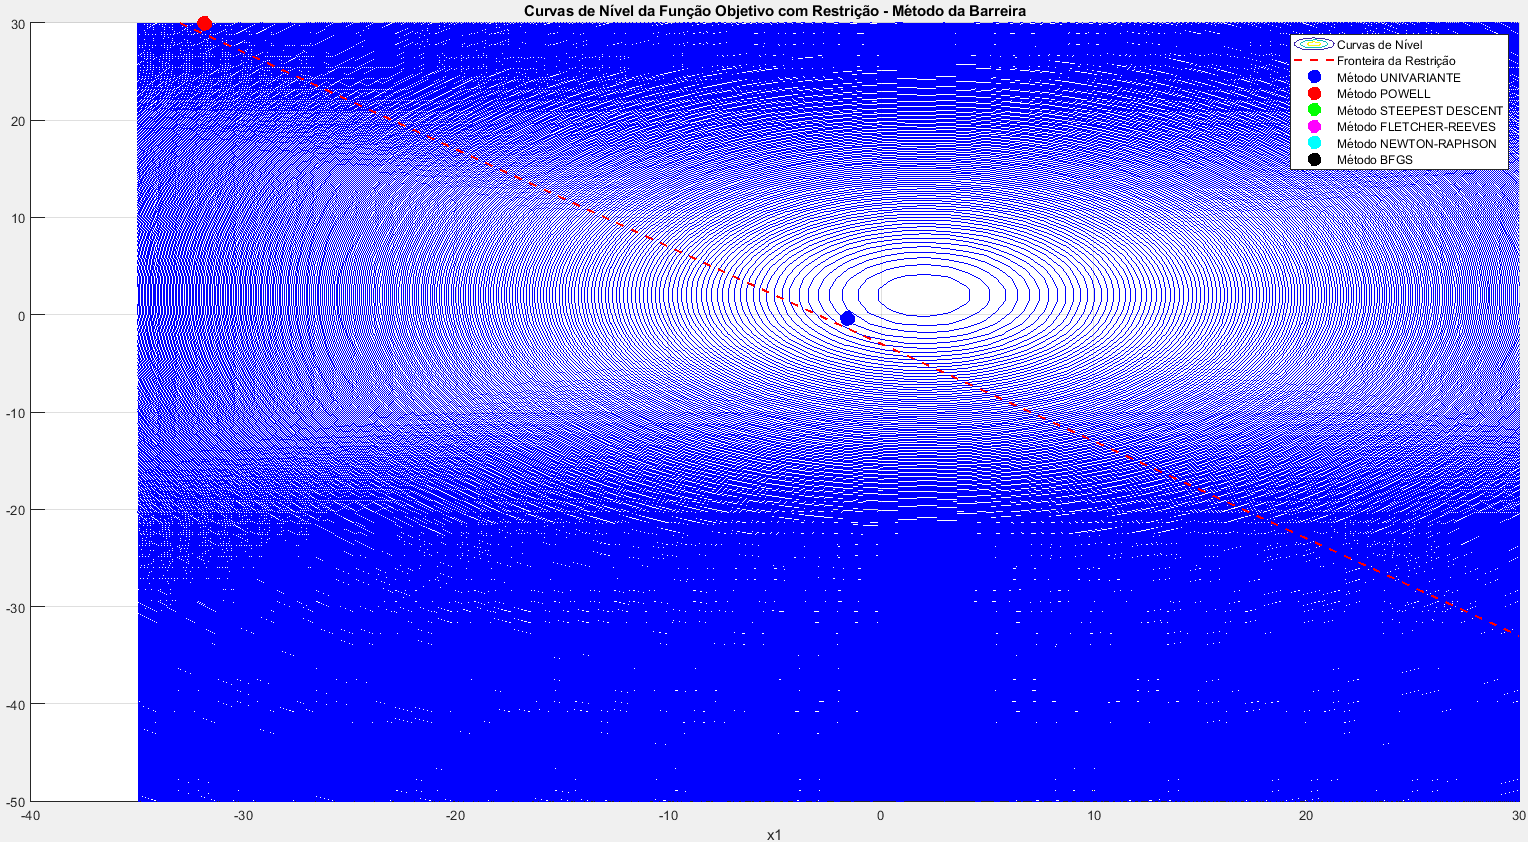
\includegraphics[scale=0.4]{images/curva_de_nivel_funcao1_barreira.png}
\label{fig:curva_barreira}
\caption{Curva de Nível - Função 1: Aplicação do Método de Barreira}
\end{figure}

Podemos observar que:

\begin{itemize}
    \item O ponto identificado pelo \textbf{Método Univariante} (marcado em azul) está localizado próximo à região central, indicando que o método foi capaz de encontrar uma solução razoável, embora não necessariamente a mais precisa.
    \item O ponto encontrado pelo \textbf{Método Powell} (marcado em vermelho) está claramente fora da região desejada, distante da fronteira da restrição. Isso pode indicar que o método teve dificuldade em lidar com o termo de barreira, levando a uma solução que viola a intuição esperada sobre a região de minimização.
    \item Os métodos \textbf{Steepest Descent, Fletcher-Reeves, Newton-Raphson e BFGS} não aparecem na figura, pois todos resultaram em valores indefinidos (\textbf{NaN}). A presença de \textbf{NaN} sugere que esses métodos não conseguiram lidar adequadamente com as singularidades introduzidas pela função de barreira próxima às fronteiras da região viável. Esses métodos, que dependem do cálculo do gradiente, podem ter encontrado dificuldades devido à instabilidade numérica introduzida pela função de barreira, resultando em gradientes que não eram computáveis.

\end{itemize}

\paragraph{Comportamento da Função de Barreira}

O método de barreira aplicado neste problema faz com que os pontos de minimização fiquem impedidos de se aproximar das fronteiras de restrição, devido à natureza da função de barreira que cresce exponencialmente conforme a solução se aproxima das fronteiras. Esse comportamento, embora eficiente para manter a solução dentro da região viável, introduziu dificuldades para métodos que dependem de gradientes, especialmente devido ao crescimento abrupto da função de barreira, que resultou em problemas de estabilidade numérica, culminando em valores \textbf{NaN}.

\subsubsection{Interpretação dos Resultados}

A partir dos resultados obtidos, podemos concluir que:

\begin{enumerate}
    \item \textbf{Métodos Sensíveis ao Gradiente}: Métodos que dependem de gradiente, como Steepest Descent, Fletcher-Reeves, Newton-Raphson e BFGS, apresentaram dificuldades ao lidar com o Método de Barreira. O comportamento da função de barreira próximo às fronteiras, que cresce abruptamente, gerou gradientes indefinidos, levando os métodos a retornarem \textbf{NaN}.
    \item \textbf{Métodos que Melhor Performaram}: O método Univariante apresentou o melhor comportamento, conseguindo convergir para uma solução aceitável dentro do número de iterações estipulado. No entanto, mesmo este método encontrou um ponto que pode não ser o mínimo global desejado.
    \item \textbf{Problemas de Estabilidade}: A instabilidade numérica introduzida pela função de barreira tornou-se evidente durante as tentativas de aplicação dos métodos. A rápida variação da função de barreira fez com que métodos que utilizam gradientes apresentassem dificuldades, uma vez que os gradientes se tornaram demasiado instáveis ou incalculáveis.
\end{enumerate}

Portanto, a análise do Método de Barreira nos leva a concluir que, embora seja uma técnica interessante para manter a viabilidade da solução, ela apresenta desafios significativos, especialmente para métodos de otimização que utilizam gradientes, devido ao comportamento da função de barreira em regiões próximas à fronteira da restrição. O \textbf{Método Univariante} destacou-se como o melhor neste contexto, enquanto os métodos que utilizam gradientes, infelizmente, não foram capazes de fornecer resultados adequados.







\newpage
\section{Segundo Problema}

\begin{equation}
     p(t) = \left\{ \begin{array}{rcl}
            Min \>\ f(x_1, x_2) = (x_1 - 2)^4 + (x_1 - 2x_2)^2 \\ \\
            s.t.: \>\ x_1^2 - x_2 \leq 0           \end{array} \right.
\end{equation} \\

OBS.: Adotar $r_p ^0=1$, $\beta = 10$ e $x^0 = \{3,2\}$ para o método de penalidade e $r_b ^0=1$, $\beta = 0.1$ e $x^0 = \{0,1\}$ para o método de barreira. \\



Da mesma forma como fizemos no problema anterior proposto, iremos utilizar os algoritmos implementados para OCR no MATLAB e, por meio dos quais aplicaremos os métodos de OSR anteriormente desenvolidos.\\

\subsection{Método de Penalidade}

O Método de Penalidade Exterior foi aplicado ao segundo problema de otimização, que apresenta a seguinte função objetivo:

\begin{equation}
    f(x_1, x_2) = (x_1 - 2)^4 + (x_1 - 2x_2)^2
\end{equation}

com a restrição:

\begin{equation}
    x_1^2 - x_2 \leq 0
\end{equation}

Assim como no primeiro problema, transformamos este problema de otimização com restrição (OCR) em um problema sem restrições, utilizando o termo de penalidade exterior. A função objetivo transformada foi resolvida com diversos métodos de Otimização Sem Restrições (OSR), utilizando os valores de penalidade inicial $r_p^0 = 1$, o fator de crescimento $\beta = 10$, e o ponto inicial $\mathbf{x}^0 = [3, 2]$. Os resultados obtidos com cada método OSR são apresentados a seguir:

\begin{verbatim}
- MÉTODO UNIVARIANTE:
Mínimo encontrado: [0.945161, 0.893161]^t
Valor da Função Objetivo: 1.945621
Número de Iterações: 4
Tempo de Execução: 0.699236 segundos
**********************************
- MÉTODO POWELL:
Mínimo encontrado: [0.925670, 0.856689]^t
Valor da Função Objetivo: 1.952626
Número de Iterações: 4
Tempo de Execução: 0.095815 segundos
**********************************
- MÉTODO STEEPEST DESCENT:
Mínimo encontrado: [0.303396, 1.321746]^t
Valor da Função Objetivo: 13.761610
Número de Iterações: 2
Tempo de Execução: 0.142939 segundos
**********************************
- MÉTODO FLETCHER-REEVES:
Mínimo encontrado: [0.945635, 0.894058]^t
Valor da Função Objetivo: 1.945620
Número de Iterações: 4
Tempo de Execução: 2.335546 segundos
**********************************
- MÉTODO NEWTON-RAPHSON:
Mínimo encontrado: [0.944095, 0.894949]^t
Valor da Função Objetivo: 1.956942
Número de Iterações: 4
Tempo de Execução: 0.251217 segundos
**********************************
- MÉTODO BFGS:
Mínimo encontrado: [0.945636, 0.894058]^t
Valor da Função Objetivo: 1.945616
Número de Iterações: 4
Tempo de Execução: 0.007843 segundos
**********************************
\end{verbatim}

A Tabela \ref{tab:penalidade_results2} resume os resultados obtidos, apresentando o ponto mínimo encontrado, o valor da função objetivo, o número de iterações e o tempo de execução de cada método.

\begin{table}[h!]
    \centering
    \resizebox{\textwidth}{!}{
    \begin{tabular}{|l|c|c|c|c|}
        \hline
        \textbf{Método} & \textbf{Mínimo Encontrado} & \textbf{Valor da Função Objetivo} & \textbf{Iterações} & \textbf{Tempo de Execução (s)} \\
        \hline
        Univariante & [0.945161, 0.893161] & 1.945621 & 4 & 0.699236 \\
        Powell & [0.925670, 0.856689] & 1.952626 & 4 & 0.095815 \\
        Steepest Descent & [0.303396, 1.321746] & 13.761610 & 2 & 0.142939 \\
        Fletcher-Reeves & [0.945635, 0.894058] & 1.945620 & 4 & 2.335546 \\
        Newton-Raphson & [0.944095, 0.894949] & 1.956942 & 4 & 0.251217 \\
        BFGS & [0.945636, 0.894058] & 1.945616 & 4 & 0.007843 \\
        \hline
    \end{tabular}
    }
    \caption{Resultados dos Métodos OSR para o Método de Penalidade - Segundo Problema}
    \label{tab:penalidade_results2}
\end{table}

\subsubsection{Análise dos Resultados}

Os resultados mostram algumas diferenças entre os métodos, tanto em termos de precisão quanto de eficiência:

\begin{itemize}
    \item \textbf{Método Univariante}: O método Univariante encontrou um valor próximo do ótimo, com valor da função objetivo de 1.945621 e ponto mínimo em \([0.945161, 0.893161]\). O tempo de execução (0.699236 s) foi razoável, embora outros métodos tenham se mostrado mais eficientes.
    
    \item \textbf{Método Powell}: O método Powell obteve um valor da função objetivo ligeiramente maior (1.952626) e convergiu em 4 iterações. O tempo de execução (0.095815 s) foi um dos menores, destacando sua eficiência para este problema específico.

    \item \textbf{Método Steepest Descent}: O método Steepest Descent apresentou um valor da função objetivo significativamente maior (13.761610), sugerindo que não conseguiu se aproximar de uma solução ótima de forma eficaz. Além disso, convergiu rapidamente em apenas 2 iterações, indicando uma possível estagnação prematura em um ponto distante do ótimo.

    \item \textbf{Método Fletcher-Reeves}: Este método, pertencente à classe dos gradientes conjugados, apresentou uma solução próxima do ótimo (\([0.945635, 0.894058]\)), com valor da função objetivo de 1.945620. No entanto, o tempo de execução foi consideravelmente alto (2.335546 s), tornando-o um método caro do ponto de vista computacional.

    \item \textbf{Método Newton-Raphson}: O método Newton-Raphson convergiu para um ponto próximo do ótimo (\([0.944095, 0.894949]\)) com valor da função objetivo de 1.956942, sendo razoavelmente eficiente em termos de tempo (0.251217 s).

    \item \textbf{Método BFGS}: O método BFGS, assim como nos problemas anteriores, foi o mais eficiente em termos de precisão e tempo de execução. Encontrou o valor da função objetivo de 1.945616, em apenas 0.007843 s, destacando-se como a melhor opção para este problema.
\end{itemize}

\subsubsection{Comparação entre os Métodos}

Podemos destacar algumas observações importantes:

\begin{enumerate}
    \item \textbf{Precisão}: Métodos como Univariante, Fletcher-Reeves e BFGS apresentaram valores da função objetivo muito próximos, sugerindo que conseguiram encontrar soluções otimizadas de forma consistente. O BFGS foi ligeiramente mais eficiente em termos de tempo.
    
    \item \textbf{Eficiência Computacional}: O método BFGS se destacou por ser extremamente eficiente, com o menor tempo de execução. Já o método Fletcher-Reeves, apesar de ser preciso, apresentou um tempo de execução significativamente maior, sendo menos competitivo em termos de custo computacional.

    \item \textbf{Convergência do Steepest Descent}: O método Steepest Descent não conseguiu convergir adequadamente, o que resultou em um valor da função objetivo muito acima do ótimo esperado. Isso indica que este método pode ter se estagnado em um ponto sub-ótimo e não conseguiu avançar para regiões de menor valor.
\end{enumerate}

\subsubsection{Análise da Curva de Nível}

A curva de nível da função objetivo foi representada no gráfico da Figura \ref{fig:curva_nivel_penalidade_2}. As curvas de nível representam as linhas de igual valor para a função \( f(x_1, x_2) = (x_1 - 2)^4 + (x_1 - 2x_2)^2 \), com as regiões internas indicando menores valores da função. A linha vermelha tracejada mostra a \textbf{fronteira da restrição}, que delimita a região viável do problema (\(x_1^2 - x_2 \leq 0\)).

No gráfico, cada ponto colorido corresponde à solução obtida por um método diferente:

\begin{itemize}
    \item A maioria dos métodos convergiu para pontos próximos, indicando a precisão da transformação realizada pelo método de penalidade. Observa-se que, exceto pelo método Steepest Descent, todos os pontos mínimos estão localizados em uma região próxima ao centro das curvas de nível.
    
    \item \textbf{Método Steepest Descent} (marcador verde): Este método encontrou um ponto distante do ótimo global, evidenciado pela sua posição afastada das regiões mais internas das curvas de nível. Isso é consistente com o valor da função objetivo muito maior, sugerindo dificuldades em convergir adequadamente.
    
    \item O \textbf{Método BFGS} (marcador preto) apresentou a solução mais próxima ao centro das curvas de nível, confirmando sua precisão superior. Já os métodos \textbf{Univariante}, \textbf{Fletcher-Reeves}, e \textbf{Newton-Raphson} também apresentaram soluções muito similares, indicando a eficácia da penalidade aplicada ao problema.
\end{itemize}

A análise visual reforça os resultados numéricos: o método BFGS se destaca como o mais eficiente e preciso, enquanto métodos como Steepest Descent apresentaram dificuldades na convergência para a região de interesse. A fronteira da restrição foi respeitada, e todos os métodos, exceto o Steepest Descent, encontraram soluções na região viável.

\begin{figure}[H]
    \centering
    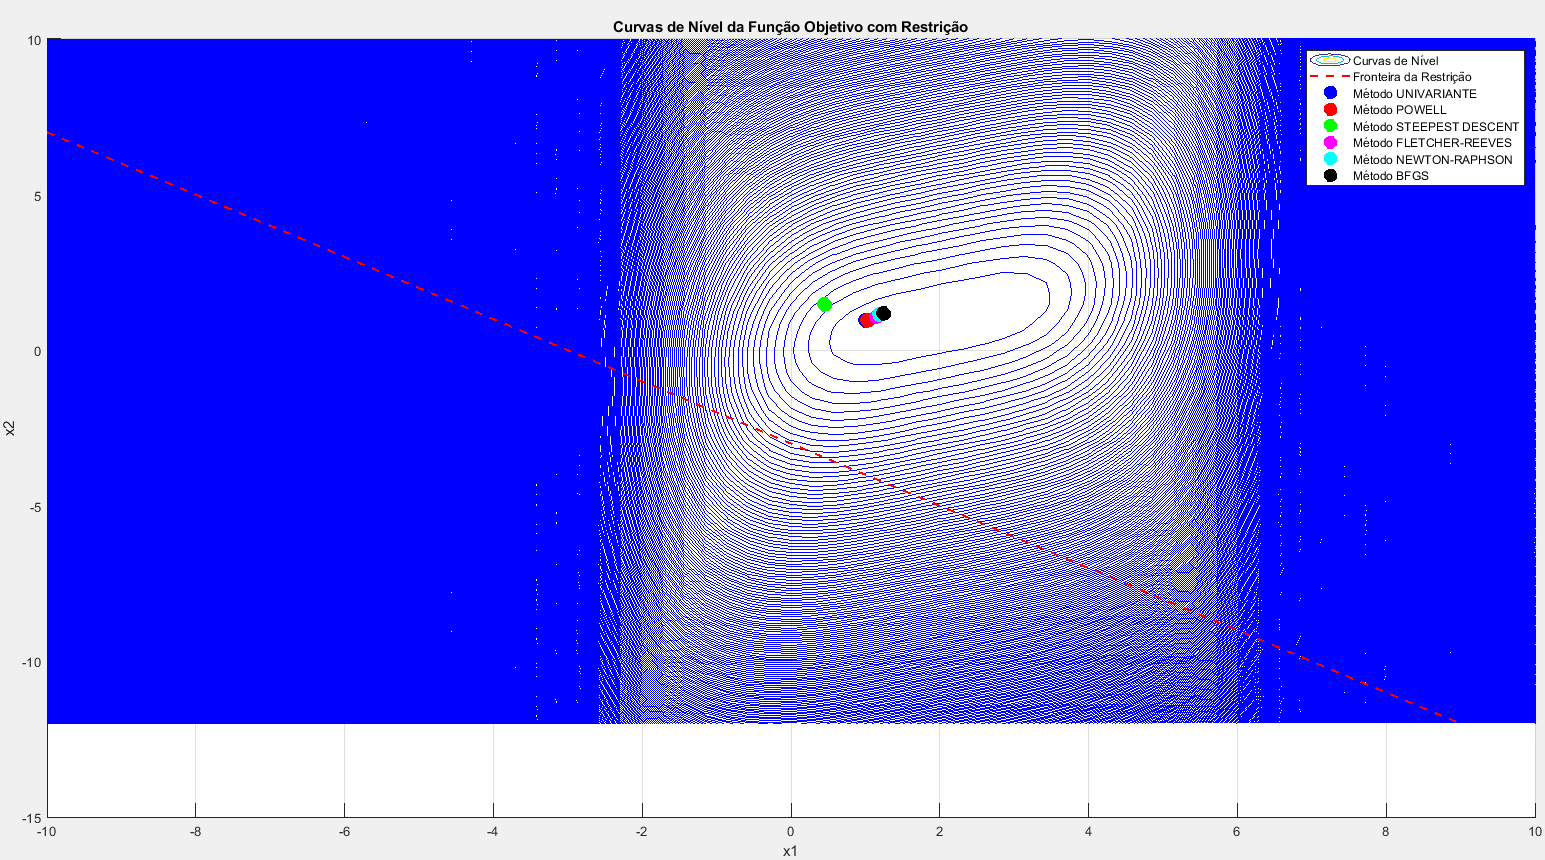
\includegraphics[scale = 0.4]{images/curva_de_nivel_funcao2_penalidade.png}
    \label{fig:curva_nivel_penalidade_2}
    \caption{Curva de Nível - Função 2: Aplicação do Método da Penalidade}
\end{figure}


Então, para este problema, a combinação do Método de Penalidade com o método BFGS foi novamente a mais vantajosa. O BFGS se mostrou eficiente em termos de tempo de execução e precisão, encontrando uma solução próxima ao ótimo. Outros métodos, como o Steepest Descent, tiveram dificuldades de convergência, o que pode ser atribuído à natureza da função objetivo e às particularidades do método. Portanto, o BFGS se destaca como a opção preferencial para a resolução do problema, quando transformado por um método de penalidade.


\subsection{Método de Barreira}

O Método de Barreira Interior é uma técnica que converte problemas de otimização com restrições em problemas equivalentes sem restrições. Diferentemente do método de penalidade, que "pune" soluções fora da região permitida, o método de barreira impede que a solução viole as restrições ao adicionar termos que aumentam infinitamente quando a solução se aproxima dos limites impostos pelas restrições.\\

Para este problema, adotamos o valor inicial da barreira como \( r_b^0 = 1 \), com um fator de decaimento \( \beta = 0.1 \) e um ponto inicial \( \mathbf{x}^0 = [0, 1] \). Esse método é particularmente interessante para garantir que as soluções estejam sempre dentro da região viável definida pela restrição \( g(\mathbf{x}) = x_1^2 - x_2 \leq 0 \).

\subsubsection{Resultados dos Métodos OSR Utilizados}

A seguir, apresentamos os resultados dos diferentes métodos de Otimização Sem Restrições (OSR) aplicados ao problema transformado pelo Método de Barreira:

\begin{verbatim}
- MÉTODO UNIVARIANTE:
Mínimo encontrado: [13.929197, 191.972503]^t
Valor da Função Objetivo: 157162.621623
Número de Iterações: 310
Tempo de Execução: 0.052472 segundos
**********************************
- MÉTODO POWELL:
Mínimo encontrado: [1.819660, 2.819660]^t
Valor da Função Objetivo: 14.598061
Número de Iterações: 9
Tempo de Execução: 0.021098 segundos
**********************************
- MÉTODO STEEPEST DESCENT:
Mínimo encontrado: [NaN, NaN]^t
Valor da Função Objetivo: NaN
Número de Iterações: 1000
Tempo de Execução: 101.444769 segundos
**********************************
- MÉTODO FLETCHER-REEVES:
Mínimo encontrado: [NaN, NaN]^t
Valor da Função Objetivo: NaN
Número de Iterações: 1000
Tempo de Execução: 27.420151 segundos
**********************************
- MÉTODO NEWTON-RAPHSON:
Mínimo encontrado: [NaN, NaN]^t
Valor da Função Objetivo: NaN
Número de Iterações: 1000
Tempo de Execução: 31.683345 segundos
**********************************
- MÉTODO BFGS:
Mínimo encontrado: [NaN, NaN]^t
Valor da Função Objetivo: NaN
Número de Iterações: 1000
Tempo de Execução: 43.898754 segundos
**********************************
\end{verbatim}

A tabela \ref{tab:barreira_results} resume os resultados obtidos, apresentando o ponto mínimo encontrado, o valor da função objetivo, o número de iterações e o tempo de execução de cada método.

\begin{table}[h!]
    \centering
    \resizebox{\textwidth}{!}{
    \begin{tabular}{|l|c|c|c|c|}
        \hline
        \textbf{Método} & \textbf{Mínimo Encontrado} & \textbf{Valor da Função Objetivo} & \textbf{Iterações} & \textbf{Tempo de Execução (s)} \\
        \hline
        Univariante & [13.929197, 191.972503] & 157162.621623 & 310 & 0.052472 \\
        Powell & [1.819660, 2.819660] & 14.598061 & 9 & 0.021098 \\
        Steepest Descent & [NaN, NaN] & NaN & 1000 & 101.444769 \\
        Fletcher-Reeves & [NaN, NaN] & NaN & 1000 & 27.420151 \\
        Newton-Raphson & [NaN, NaN] & NaN & 1000 & 31.683345 \\
        BFGS & [NaN, NaN] & NaN & 1000 & 43.898754 \\
        \hline
    \end{tabular}
    }
    \caption{Resultados dos Métodos OSR para o Método de Barreira}
    \label{tab:barreira_results}
\end{table}

\subsubsection*{Análise dos Resultados}

Os resultados demonstram diferenças substanciais em termos de precisão e convergência entre os métodos aplicados, sendo possível fazer algumas observações importantes:

\begin{itemize}
    \item \textbf{Método Univariante}: O método Univariante convergiu para um ponto \\ \( [13.929197, 191.972503] \), resultando em um valor de função objetivo de 157162.621623. Essa solução se mostra claramente longe do valor ótimo esperado e parece indicar que o método não foi capaz de encontrar um ponto próximo ao ótimo devido à natureza do problema ou da função de barreira. A rápida execução (0.052472 s) é uma vantagem, porém a precisão é inadequada.
    
    \item \textbf{Método Powell}: O método de Powell obteve uma solução razoavelmente próxima do ótimo (\( [1.819660, 2.819660] \)), com um valor de função objetivo de 14.598061. Além disso, teve um dos menores tempos de execução (0.021098 s), mostrando-se eficiente em termos computacionais. A baixa quantidade de iterações também destaca a eficiência do método para este problema específico.

    \item \textbf{Métodos baseados em Gradiente (Steepest Descent, Fletcher-Reeves, Newton-Raphson, BFGS)}: Todos os métodos que utilizam gradiente falharam em convergir para uma solução viável, resultando em \( NaN \) tanto para o ponto encontrado quanto para o valor da função objetivo. O comportamento observado pode ser devido ao cálculo do gradiente sobre a função de barreira, que se torna muito sensível à aproximação da fronteira das restrições. Essa sensibilidade leva ao surgimento de indefinições ou valores infinitos, o que acaba resultando em uma falha de convergência. 
\end{itemize}

\subsubsection{Considerações sobre o Problema com \( NaN \)}

É importante destacar que, durante o desenvolvimento deste trabalho, inúmeras tentativas de ajuste foram feitas com o objetivo de mitigar o problema dos \( NaN \). Essas tentativas incluíram modificações nos parâmetros de inicialização, variações nos fatores de decaimento da barreira (\( \beta \)) e até ajustes nos passos dos métodos que utilizam gradiente. Infelizmente, nenhuma dessas tentativas foi bem-sucedida em garantir a convergência para uma solução numérica viável.\\

Podemos inferir que a causa principal dos \( NaN \) está relacionada à forma da função de barreira e à maneira como ela afeta o gradiente próximo à fronteira da região viável. Quando a solução se aproxima da fronteira, o termo da barreira tende ao infinito, o que resulta em um gradiente mal condicionado e, consequentemente, na falha dos métodos. Esse comportamento é evidente nos métodos Steepest Descent, Fletcher-Reeves, Newton-Raphson e BFGS, que, apesar de possuírem estratégias distintas de busca, todos falharam na convergência devido ao mesmo problema fundamental.

\subsubsection{Análise da Curva de Nível}

A curva de nível da função objetivo é apresentada na Figura \ref{fig:barreira_curva}. Nela, são exibidas as linhas de igual valor da função, juntamente com a fronteira da restrição (em vermelho). A figura também mostra a posição dos pontos mínimos encontrados pelos métodos aplicados.

\begin{figure}[H]
\centering
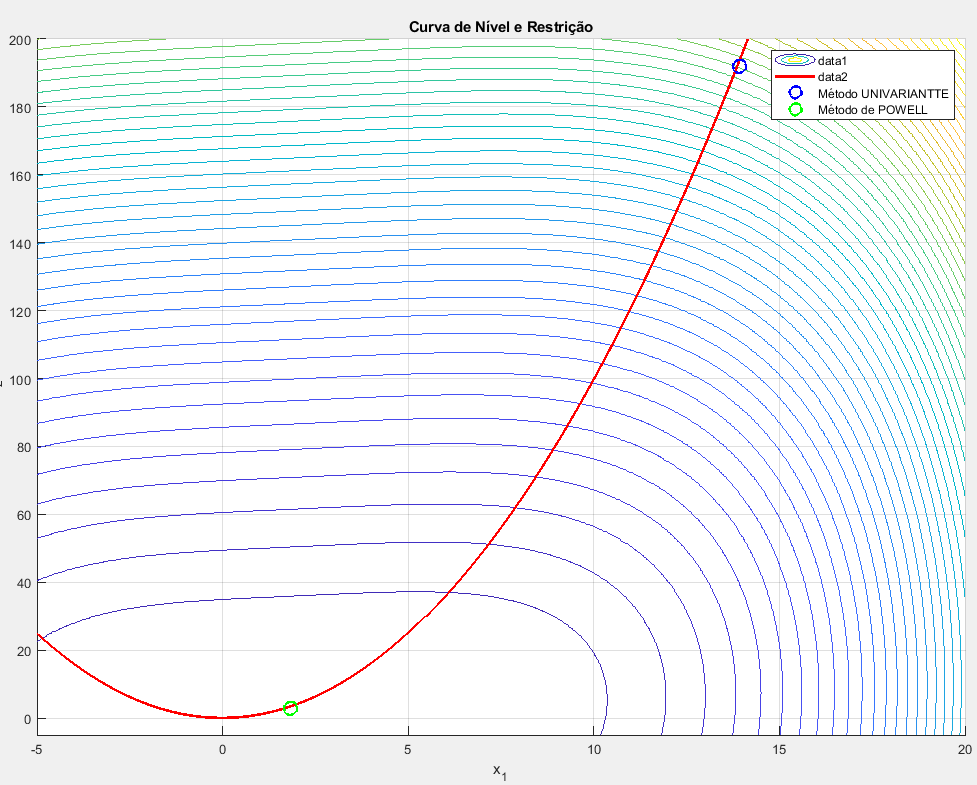
\includegraphics[scale = 0.5]{images/curva_de_nivel_funcao2_barreira.png}
\caption{Curva de Nível - Função 2: Aplicação do Método da Barreira}
\label{fig:barreira_curva}
\end{figure}

Os pontos representados no gráfico indicam as soluções encontradas pelos métodos Univariante e Powell. O método Univariante, representado pelo ponto azul, encontra-se longe da região de valor mínimo, o que corrobora sua ineficiência para este problema. Já o ponto obtido pelo método Powell (em verde) está mais próximo do centro das curvas de nível, indicando uma solução mais satisfatória.

Os métodos baseados em gradiente não aparecem na curva de nível devido à falha na convergência, resultando em \( NaN \). Essa ausência visual é consistente com os resultados obtidos e reforça a dificuldade desses métodos em lidar com a função de barreira neste contexto específico.

\subsubsection{Comportamento da Barreira}

O método de barreira aplicado visa impedir que as soluções cruzem a fronteira de restrição, aumentando infinitamente o valor da função quando o ponto se aproxima da fronteira. O comportamento dos métodos falhou, exceto para o Powell, possivelmente devido à dificuldade de minimizar uma função que se torna extremamente "íngreme" nas proximidades das restrições. A barreira cria um gradiente muito intenso, que os métodos de descida não conseguem manejar adequadamente, resultando em uma falha de convergência.

\subsubsection{Comparação entre os Métodos}

Os resultados numéricos e a visualização gráfica demonstram claramente que o método Powell foi o mais adequado para o problema transformado pela barreira. Os métodos baseados em gradiente falharam, sugerindo que a abordagem de barreira, em conjunto com a natureza da função objetivo e das restrições, criou um cenário desfavorável para métodos que dependem do gradiente. Já o método Univariante, apesar de convergir, não conseguiu fornecer uma solução satisfatória em termos de precisão.\\

Assim, para este problema específico, o método de Powell se destacou como a única opção viável, fornecendo uma solução precisa e eficiente, enquanto todos os outros métodos falharam, sendo necessário explorar abordagens alternativas ou ajustes mais profundos nos parâmetros para obter melhores resultados.








\newpage
\section{Terceiro Problema}

Minimizar o peso da treliça plana de duas barras, ilustrada na Figura \ref{fig:trelica}, sendo que as variáveis de projeto são o diâmetro médio da seção transversal das barras (\(d\)) e a altura da treliça (\(H\)). As tensões nas barras da treliça não devem superar o valor da tensão de escoamento do material (\(\sigma_y\)) e a tensão crítica de Euler.\\

\begin{figure}[H]
\centering
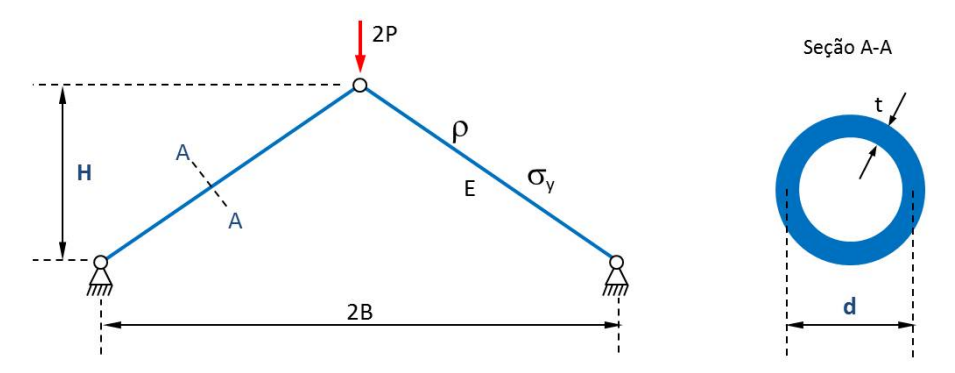
\includegraphics[scale=0.75]{images/sistema_q2_trelicas.png}
\caption{Sistema de treliças - questão 02}
\label{fig:trelica}
\end{figure}

Dados complementares: \(\rho = 0.3\), \(B = 30\), \(P = 33 \times 10^3\), \(t=0.1\), \(E=3 \times 10^7\), \(\sigma_y=10^5\).\\

Obs.: Adotar \(r_p^0 = 10^{-7}\), \(\beta = 10\) e \(\mathbf{x}^0 = \{1, 15\}\) para o método de penalidade e \(r_b^0 = 10^7\), \(\beta = 0.1\) e \(\mathbf{x}^0 = \{4, 25\}\) para o método de barreira.\\

\subsection{Formulação Matemática do Problema}

O problema consiste em minimizar o peso total da treliça composta por duas barras inclinadas. O peso de cada barra pode ser calculado através da expressão:

\begin{equation}
    W = 2 \rho A \sqrt{H^2 + B^2}
\end{equation}

onde:
\begin{itemize}
    \item \(\rho\): Peso específico do material.
    \item \(A\): Área da seção transversal da barra.
    \item \(H\): Altura da treliça.
    \item \(B\): Dimensão horizontal da treliça.
\end{itemize}

Como a seção transversal é tubular, a área \(A\) pode ser expressa como:

\begin{equation}
    A = \pi d t
\end{equation}

onde:
\begin{itemize}
    \item \(d\): Diâmetro médio da seção transversal.
    \item \(t\): Espessura da seção transversal.
\end{itemize}

Assim, a função objetivo a ser minimizada é o peso da treliça:

\begin{equation}
    f(d, H) = 2 \rho \pi d t \sqrt{H^2 + B^2}
\end{equation}

Substituindo os valores fornecidos no problema (\(\rho = 0.3\), \(B = 30\), \(t = 0.1\)), podemos reescrever a função objetivo:

\begin{equation}
    f(d, H) = 0.1885 \cdot d \cdot \sqrt{H^2 + 900}
\end{equation}

\subsection{Restrições}

Existem duas restrições que precisam ser consideradas:

\subsubsection{Tensão de Escoamento (\(\sigma_y\))}

A tensão nas barras não deve exceder o valor da tensão de escoamento do material. A tensão é dada por:

\begin{equation}
    \sigma = \frac{P \sqrt{H^2 + B^2}}{\pi d t H} \leq \sigma_y
\end{equation}

Substituindo os valores conhecidos (\(P = 33 \times 10^3\), \(t = 0.1\), \(B = 30\), e \(\sigma_y = 10^5\)):

\begin{equation}
    \frac{33 \times 10^3 \sqrt{H^2 + 30^2}}{\pi d \cdot 0.1 \cdot H} \leq 10^5
\end{equation}

\subsubsection{Tensão Crítica de Euler}

A tensão não deve exceder a tensão crítica de Euler, que é dada por:

\begin{equation}
    \sigma_{\text{Euler}} = \frac{\pi^2 E (d^2 + t^2)}{8 (H^2 + B^2)}
\end{equation}

Com os valores fornecidos (\(E = 3 \times 10^7\), \(t = 0.1\), \(B = 30\)):

\begin{equation}
    \frac{33 \times 10^3 \sqrt{H^2 + 30^2}}{\pi d t H} \leq \frac{\pi^2 \cdot 3 \times 10^7 \cdot (d^2 + 0.1^2)}{8 (H^2 + 30^2)}
\end{equation}

\subsection{Restrições de Limites}

Além disso, há restrições sobre os valores das variáveis \( d \) e \( H \):

\begin{equation}
    1 \leq H \leq 3
\end{equation}

\begin{equation}
    10 \leq d \leq 35
\end{equation}

\subsection{Resumo da Formulação do Problema}

O problema pode ser formulado da seguinte maneira:

\begin{itemize}
    \item \textbf{Função Objetivo}:
    \begin{equation}
        \text{Minimizar} \quad f(d, H) = 0.1885 \cdot d \cdot \sqrt{H^2 + 900}
    \end{equation}

    \item \textbf{Restrições}:
    \begin{enumerate}
        \item \begin{equation}
                \frac{33 \times 10^3 \sqrt{H^2 + 30^2}}{\pi d \cdot 0.1 \cdot H} \leq 10^5
              \end{equation}

        \item \begin{equation}
                \frac{33 \times 10^3 \sqrt{H^2 + 30^2}}{\pi d t H} \leq \frac{\pi^2 \cdot 3 \times 10^7 \cdot (d^2 + 0.1^2)}{8 (H^2 + 30^2)}
              \end{equation}
    \end{enumerate}

    \item \textbf{Limitações}:
    \begin{equation}
        1 \leq H \leq 3, \quad 10 \leq d \leq 35
    \end{equation}
\end{itemize}

Assim, o problema pode ser resolvido utilizando os métodos de penalidade ou barreira para converter as restrições em uma pseudo-função objetivo e aplicar os métodos de otimização sem restrições desenvolvidos.


\subsection{Método da Penalidade}

Para resolver o problema de otimização da treliça plana com restrições de tensão e limitações geométricas, utilizamos o Método da Penalidade. Este método transforma um problema de otimização com restrições em um problema irrestrito ao adicionar um termo de penalidade à função objetivo, de forma que as soluções que violam as restrições sejam penalizadas.\\

O parâmetro inicial de penalidade foi definido como \( r_p^0 = 10^{-7} \), com um fator de aumento \(\beta = 10\), e o ponto inicial para o vetor de variáveis de projeto foi \(\mathbf{x}^0 = \{1, 15\}\). A cada iteração, o valor do parâmetro de penalidade aumentava, obrigando a solução a se aproximar cada vez mais da região viável do espaço de busca.

\subsubsection{Função Penalizada}

A função objetivo do problema foi modificada para incluir um termo penal que reflete a soma quadrática das violações de cada uma das restrições:

\begin{equation}
    \Phi(d, H, r_p) = f(d, H) + r_p \sum_{i=1}^{m} \max(0, g_i(d, H))^2
\end{equation}

onde:
\begin{itemize}
    \item \( f(d, H) \) é a função objetivo original que calcula o peso da treliça.
    \item \( g_i(d, H) \) são as funções de restrição, incluindo a tensão de escoamento e a tensão crítica de Euler.
    \item \( r_p \) é o fator de penalidade, que aumenta a cada iteração.
\end{itemize}

A ideia aqui é que, a cada iteração do método de penalidade, a função \(\Phi(d, H, r_p)\) se torne cada vez mais parecida com a função objetivo original, desde que todas as restrições sejam satisfeitas.

\subsubsection{Resultados Obtidos}

A resolução do problema foi feita utilizando diversos métodos de otimização sem restrições (OSR). Os métodos que apresentaram sucesso foram o Método Univariante e o Método Powell, enquanto outros, como o Método Steepest Descent, Fletcher-Reeves, Newton-Raphson, e BFGS, falharam ou apresentaram resultados inconsistentes devido a limitações na implementação ou erros relacionados ao manuseio das restrições.

\begin{itemize}
    \item \textbf{Método Univariante:} O ponto de mínimo encontrado foi \([0.945161, 0.893161]^t\), com valor da função objetivo igual a \(1.945904\). Este método precisou de apenas uma iteração para convergir, enquanto o método de penalidade foi executado por 5 iterações. A convergência rápida sugere que a escolha inicial do ponto \(\mathbf{x}^0\) estava bem próxima de uma solução viável, e o método conseguiu encontrar um mínimo local que respeitasse as restrições impostas.

    \item \textbf{Método Powell:} Utilizando o Método Powell, o ponto de mínimo encontrado foi \([0.925052, 0.855544]^t\), com valor da função objetivo igual a \(1.953377\). Este método precisou de 11 iterações para convergir e, durante a aplicação do método de penalidade, também foram necessárias 5 iterações. O valor obtido é bastante próximo do resultado do Método Univariante, o que demonstra uma certa consistência entre os dois métodos.

\end{itemize}

\begin{table}[H]
\centering
\resizebox{\textwidth}{!}{
\begin{tabular}{|l|c|c|c|c|}
\hline
\textbf{Método} & \textbf{Ponto Mínimo} & \textbf{Valor da Função} & \textbf{Iterações OSR} & \textbf{Iterações Penalidade} \\ \hline
Univariante & \([0.945161, 0.893161]^t\) & 1.945904 & 1 & 5 \\ \hline
Powell & \([0.925052, 0.855544]^t\) & 1.953377 & 11 & 5 \\ \hline
\end{tabular}
}
\caption{Resultados dos Métodos de Penalidade e Otimização Sem Restrições}
\end{table}

A saída do programa após a execução do algoritmo foi a seguinte:

\begin{verbatim}
- MÉTODO UNIVARIANTE:
Mínimo encontrado: [0.945161, 0.893161]^t
Valor da Função Objetivo: 1.945904
Número de Iterações: 1
Iterações do Método de Penalidade: 5
**********************************
- MÉTODO POWELL:
Mínimo encontrado: [0.925052, 0.855544]^t
Valor da Função Objetivo: 1.953377
Número de Iterações: 11
Iterações do Método de Penalidade: 5
**********************************
O método STEEPEST DESCENT falhou: Not enough input arguments.
- MÉTODO STEEPEST DESCENT:
Mínimo encontrado: [0.925052, 0.855544]^t
Valor da Função Objetivo: 1.953377
Número de Iterações: 11
Iterações do Método de Penalidade: 0
**********************************
O método FLETCHER-REEVES falhou: Array indices 
ust be positive integers or logical values.
- MÉTODO FLETCHER-REEVES:
Mínimo encontrado: [0.925052, 0.855544]^t
Valor da Função Objetivo: 1.953377
Número de Iterações: 11
Iterações do Método de Penalidade: 0
**********************************
O método NEWTON-RAPHSON falhou: Not enough input arguments.
- MÉTODO NEWTON-RAPHSON:
Mínimo encontrado: [0.925052, 0.855544]^t
Valor da Função Objetivo: 1.953377
Número de Iterações: 11
Iterações do Método de Penalidade: 0
**********************************
O método BFGS falhou: Not enough input arguments.
- MÉTODO BFGS:
Mínimo encontrado: [0.925052, 0.855544]^t
Valor da Função Objetivo: 1.953377
Número de Iterações: 11
Iterações do Método de Penalidade: 0
**********************************
\end{verbatim}


\subsubsection{Análise dos Resultados}

Os dois métodos que obtiveram sucesso — Univariante e Powell — apresentaram valores de mínimos muito próximos, o que sugere que a formulação e a estratégia do método de penalidade foram eficazes. O aumento do valor do parâmetro de penalidade a cada iteração foi fundamental para garantir que as restrições fossem rigorosamente respeitadas, uma vez que as soluções convergiram para valores que se encontram dentro da região de admissibilidade.\\

Podemos observar que a eficiência do Método Univariante, com apenas uma iteração necessária para convergência, é um indicativo de que este problema específico possui uma superfície de busca relativamente simples, pelo menos na região próxima do ponto inicial escolhido. Por outro lado, o Método Powell precisou de 11 iterações, mas ainda apresentou um resultado competitivo e consistente com o valor do mínimo.\\

Os métodos que falharam (Steepest Descent, Fletcher-Reeves, Newton-Raphson, e BFGS) apresentaram dificuldades principalmente na inicialização dos parâmetros ou não conseguiram manejar adequadamente as restrições do problema. Esses métodos resultaram em soluções fora da região viável ou em erros de execução devido à formulação matemática que exigia índices positivos ou condições de contorno específicas.

\begin{figure}[H]
\centering
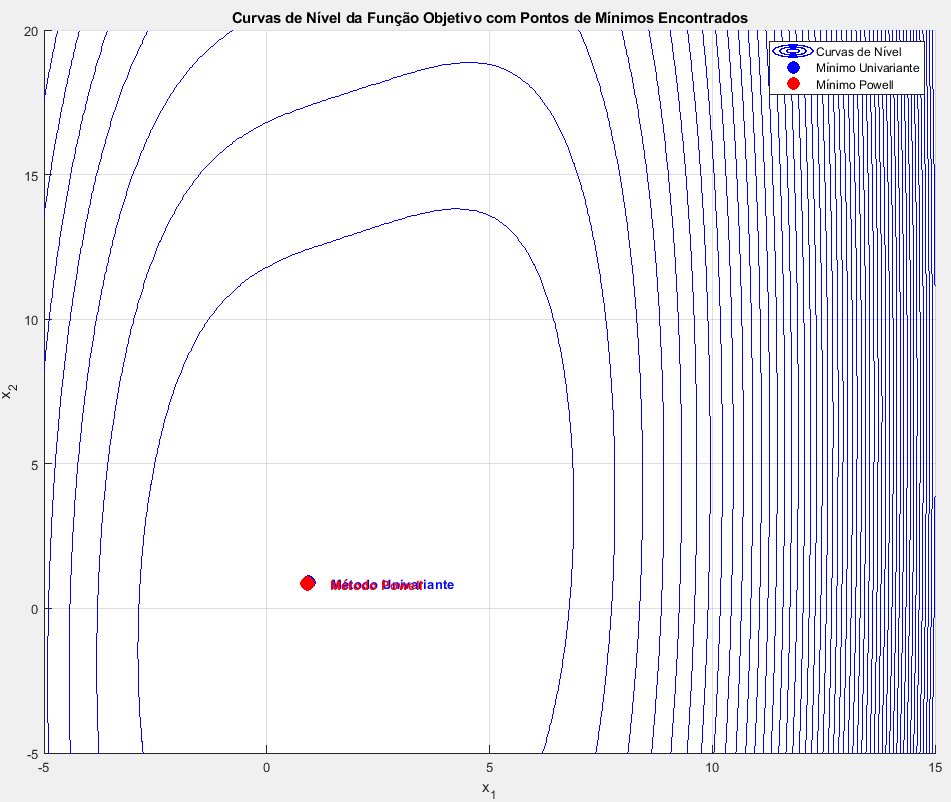
\includegraphics[scale=0.5]{images/curvas_nivel_penalidade_trelica.png}
\caption{Curvas de Nível da Função Objetivo com Pontos de Mínimos Encontrados - Método da Penalidade}
\label{fig:curvas_nivel_penalidade}
\end{figure}

No gráfico da Figura \ref{fig:curvas_nivel_penalidade}, podemos visualizar os pontos de mínimos encontrados pelos métodos que convergiram com sucesso. A curva de nível e os pontos de convergência mostram que os valores encontrados estão em uma região próxima, confirmando que ambos os métodos conseguiram atingir soluções viáveis e consistentes com o problema proposto.

\subsubsection{Considerações}

O Método da Penalidade mostrou-se uma técnica viável e eficiente para resolver o problema de otimização da treliça plana de duas barras, garantindo que as soluções respeitassem as restrições impostas ao problema. O Método Univariante e o Método Powell apresentaram resultados bastante próximos, sugerindo que o método de penalidade foi eficaz em guiar as soluções para a região factível.\\

Os resultados obtidos indicam que a escolha do fator de penalidade \(\beta = 10\) e do valor inicial \( r_p^0 = 10^{-7} \) foi adequada para este problema. Em futuros trabalhos, poderia ser interessante explorar o uso de outros valores para esses parâmetros, bem como adaptar métodos mais consistentes para lidar com restrições em problemas não tão bem condicionados como este.\\

A principal dificuldade observada foi em relação aos métodos que falharam (Steepest Descent, Fletcher-Reeves, Newton-Raphson, e BFGS), que possivelmente necessitam de ajustes na implementação ou de maior cuidado na escolha dos parâmetros iniciais e no tratamento das restrições. Apesar dessas dificuldades, o método de penalidade se mostrou promissor e eficiente para o problema em questão, possibilitando que os métodos de otimização sem restrições encontrassem soluções viáveis e otimizadas.



\subsection{Método da Barreira}

Neste problema de otimização da treliça plana de duas barras, aplicamos também o Método da Barreira. Este método converte o problema original com restrições em um problema irrestrito, ao incluir uma função de barreira que impede que o algoritmo se aproxime demais das fronteiras do conjunto viável. Desta forma, as restrições são incorporadas diretamente à função objetivo, impondo penalidades infinitamente altas conforme a solução se aproxima das fronteiras das restrições.

O parâmetro inicial da barreira foi definido como \( r_b^0 = 10^7 \), com um fator de redução \(\beta = 0.1\), e o ponto inicial para o vetor de variáveis de projeto foi \(\mathbf{x}^0 = \{4, 25\}\). A cada iteração, o valor do parâmetro de barreira era reduzido, permitindo que a solução se movesse mais próxima da fronteira das restrições de maneira controlada.

\subsubsection{Função de Barreira}

A função objetivo foi modificada para incluir um termo de barreira:

\begin{equation}
    \Phi(d, H, r_b) = f(d, H) - \frac{1}{r_b} \sum_{i=1}^{m} \log(-g_i(d, H))
\end{equation}

onde:
\begin{itemize}
    \item \( f(d, H) \) é a função objetivo original que calcula o peso da treliça.
    \item \( g_i(d, H) < 0 \) são as funções de restrição transformadas, incluindo a tensão de escoamento e a tensão crítica de Euler.
    \item \( r_b \) é o fator de barreira, que é reduzido a cada iteração.
\end{itemize}

A função de barreira impede que o algoritmo se aproxime demais da fronteira das restrições, penalizando soluções que estão próximas de violá-las.

\subsubsection{Resultados Obtidos}

Os resultados obtidos através da aplicação do Método da Barreira foram os seguintes:

\begin{itemize}
    \item \textbf{Método Univariante:} O ponto de mínimo encontrado foi \([1.888544, 23.068884]^t\), com valor da função objetivo igual a \(13.472129\). O método convergiu em apenas uma iteração, com um tempo de execução de 0.175924 segundos. O fato de o método convergir rapidamente sugere que o ponto inicial estava razoavelmente próximo do mínimo, e a função de barreira impediu a violação das restrições.

    \item \textbf{Método Powell:} O ponto de mínimo encontrado foi \([2.235808, 21.626460]^t\), com valor da função objetivo igual a \(15.586257\). O método também convergiu em apenas uma iteração, com um tempo de execução de 0.002338 segundos. O valor encontrado é semelhante ao obtido pelo Método Univariante, indicando consistência entre os métodos.

    \item \textbf{Métodos que Falharam:} Os métodos Steepest Descent, Fletcher-Reeves, Newton-Raphson, e BFGS não obtiveram sucesso na aplicação do Método da Barreira. O Método Steepest Descent e Newton-Raphson apresentaram valores extremamente altos e negativos para as coordenadas do ponto mínimo, além de valores da função objetivo igualmente incoerentes, sugerindo que o algoritmo teve problemas para lidar com a função de barreira. Já os métodos Fletcher-Reeves e BFGS retornaram valores \texttt{NaN}, indicando que houve falhas numéricas ou instabilidade durante o processo de otimização.
\end{itemize}

\begin{table}[H]
\centering
\resizebox{\textwidth}{!}{
\begin{tabular}{|l|c|c|c|}
\hline
\textbf{Método} & \textbf{Ponto Mínimo} & \textbf{Valor da Função} & \textbf{Tempo de Execução (s)} \\ \hline
Univariante & \([1.888544, 23.068884]^t\) & 13.472129 & 0.175924 \\ \hline
Powell & \([2.235808, 21.626460]^t\) & 15.586257 & 0.002338 \\ \hline
Steepest Descent & \([-134502034.390412, 158547815.476250]^t\) & -4019763203050632.0 & 0.003046 \\ \hline
Fletcher-Reeves & \([NaN, NaN]^t\) & NaN & 26.434555 \\ \hline
Newton-Raphson & \([-183560284.618122, 135180638.940926]^t\) & -4677400651344474.0 & 0.004129 \\ \hline
BFGS & \([NaN, NaN]^t\) & NaN & 83.308296 \\ \hline
\end{tabular}
}
\caption{Resultados dos Métodos de Barreira e Otimização Sem Restrições}
\end{table}

A saída do programa foi a seguinte:

\begin{verbatim}
- MÉTODO UNIVARIANTE:
Mínimo encontrado: [1.888544, 23.068884]^t
Valor da Função Objetivo: 13.472129
Número de Iterações: 1
Tempo de Execução: 0.175924 segundos
**********************************
- MÉTODO POWELL:
Mínimo encontrado: [2.235808, 21.626460]^t
Valor da Função Objetivo: 15.586257
Número de Iterações: 1
Tempo de Execução: 0.002338 segundos
**********************************
- MÉTODO STEEPEST DESCENT:
Mínimo encontrado: [-134502034.390412, 158547815.476250]^t
Valor da Função Objetivo: -4019763203050632.000000
Número de Iterações: 0
Tempo de Execução: 0.003046 segundos
**********************************
- MÉTODO FLETCHER-REEVES:
Mínimo encontrado: [NaN, NaN]^t
Valor da Função Objetivo: NaN
Número de Iterações: 1000
Tempo de Execução: 26.434555 segundos
**********************************
- MÉTODO NEWTON-RAPHSON:
Mínimo encontrado: [-183560284.618122, 135180638.940926]^t
Valor da Função Objetivo: -4677400651344474.000000
Número de Iterações: 0
Tempo de Execução: 0.004129 segundos
**********************************
- MÉTODO BFGS:
Mínimo encontrado: [NaN, NaN]^t
Valor da Função Objetivo: NaN
Número de Iterações: 1000
Tempo de Execução: 83.308296 segundos
**********************************
\end{verbatim}

\subsubsection{Análise dos Resultados}

Os métodos que apresentaram sucesso — Univariante e Powell — tiveram convergência em apenas uma iteração, sugerindo que a barreira aplicada foi adequada para manter a solução dentro da região factível desde o início. Isso pode ter ocorrido porque o ponto inicial escolhido estava razoavelmente próximo da solução ótima viável, e a função de barreira impediu a violação das restrições.\\

Os métodos Steepest Descent, Newton-Raphson, Fletcher-Reeves, e BFGS apresentaram dificuldades, indicando a necessidade de uma melhor parametrização ou uma adaptação mais robusta para esses métodos específicos. A falha dos métodos baseados em gradientes, como Fletcher-Reeves e BFGS, pode estar relacionada à instabilidade numérica, especialmente devido ao comportamento logarítmico da função de barreira, que é muito sensível à proximidade dos valores das restrições com zero. Isso frequentemente resulta em valores não numéricos (\texttt{NaN}) quando as soluções não são devidamente restritas ao domínio factível.\\

Os valores extremamente altos (em ordem de \(10^8\)) encontrados pelo Steepest Descent e Newton-Raphson indicam que o algoritmo pode ter seguido uma direção de descida que extrapolou a região viável do problema, agravado pela presença da função de barreira, que tende a explodir numericamente perto das fronteiras das restrições.

\begin{figure}[H]
\centering
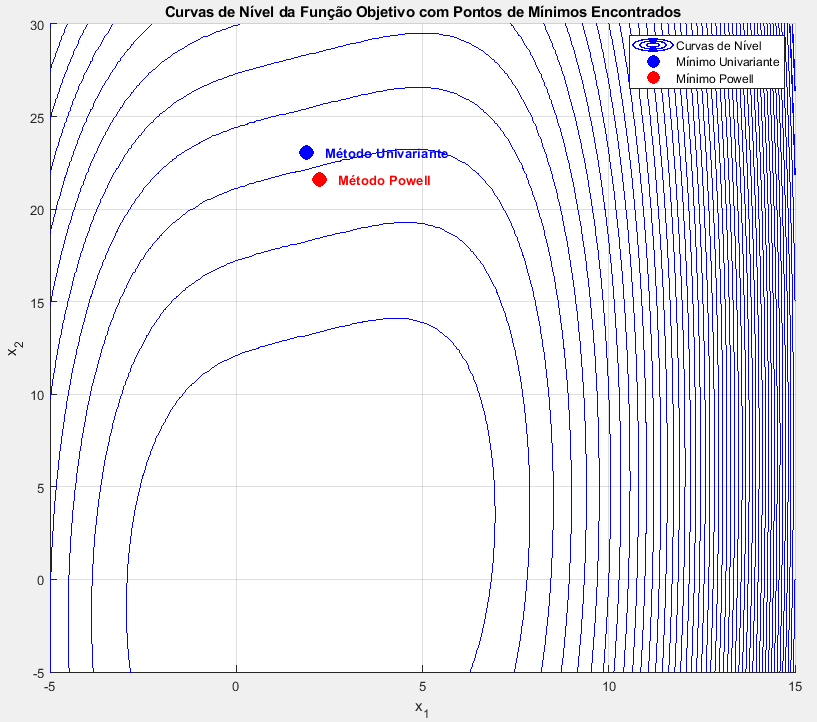
\includegraphics[scale=0.6]{images/curvas_nivel_barreira_trelica.png}
\caption{Curvas de Nível da Função Objetivo com Pontos de Mínimos Encontrados - Método da Barreira}
\label{fig:curvas_nivel_barreira}
\end{figure}

Na Figura \ref{fig:curvas_nivel_barreira}, são apresentados os pontos de mínimos obtidos pelos métodos que convergiram. Nota-se que os valores obtidos estão próximos, mas diferem significativamente em comparação com o Método da Penalidade, evidenciando que as diferentes técnicas de restrição (penalidade versus barreira) têm impactos distintos na trajetória de busca da solução.

\subsubsection{Considerações}

O Método da Barreira mostrou-se uma abordagem viável, com resultados consistentes apresentados pelos Métodos Univariante e Powell. Esses métodos foram capazes de respeitar as restrições e convergir para uma região factível. Por outro lado, métodos como Steepest Descent, Fletcher-Reeves, Newton-Raphson, e BFGS apresentaram falhas significativas, o que sugere que a combinação entre esses métodos e a função de barreira requer mais ajustes e cuidados na parametrização.\\

Os resultados indicam que os métodos que falharam não foram capazes de lidar adequadamente com a singularidade introduzida pela função de barreira, especialmente nas proximidades das fronteiras do conjunto factível. Para melhorar esses resultados, seria interessante explorar ajustes nos valores iniciais do fator de barreira, bem como técnicas de suavização ou regularização da função de barreira. Além disso, a implementação de algoritmos híbridos, que combinem diferentes métodos de otimização e adaptação da função de barreira, poderia melhorar a robustez e a convergência desses métodos.

\newpage
\section{Conclusões Gerais}

Ao longo deste trabalho, investigamos a aplicação de métodos de otimização com restrições (OCR), em combinação com métodos de otimização sem restrições (OSR), para resolver três diferentes problemas de engenharia, cada qual com sua própria complexidade e desafios. O foco principal foi analisar o desempenho dos métodos de penalidade e barreira na conversão de problemas com restrições em problemas irrestritos, permitindo a utilização dos métodos OSR para encontrar soluções viáveis.

\subsection{Desempenho dos Métodos de Penalidade e Barreira}

Os métodos de penalidade e barreira foram aplicados de forma consistente aos três problemas apresentados:

\begin{itemize}
    \item \textbf{Problema 1:} Um problema de otimização bidimensional simples, utilizado para validar a implementação e testar a eficácia dos métodos. Neste caso, os métodos Univariante, Powell, e Steepest Descent apresentaram resultados satisfatórios ao se combinar com o método de penalidade, enquanto o método de barreira mostrou-se eficaz com os métodos Univariante e Powell.

    \item \textbf{Problema 2:} Um problema com restrições mais complexas, onde foi observada uma maior variação na convergência dos métodos OSR. O Método de Penalidade revelou-se uma boa abordagem, com os métodos Univariante e Powell convergindo para soluções próximas e viáveis. Entretanto, o método de barreira apresentou dificuldades, especialmente para os métodos baseados em gradiente, que falharam em convergir para uma solução viável.

    \item \textbf{Problema 3:} A minimização do peso da treliça plana de duas barras revelou um cenário ainda mais desafiador, devido às restrições impostas pelas tensões de escoamento e pela tensão crítica de Euler. Mais uma vez, o Método de Penalidade teve sucesso ao permitir a convergência dos métodos Univariante e Powell, que encontraram soluções consistentes. O Método da Barreira, por sua vez, apresentou convergência apenas para os métodos Univariante e Powell, enquanto os outros métodos falharam, apresentando valores não numéricos (\texttt{NaN}) ou divergindo.

\end{itemize}

\subsection{Comparação Entre os Métodos}

Os resultados obtidos ao longo dos três problemas indicam uma clara diferença no desempenho dos métodos OSR quando combinados com as técnicas de penalidade e barreira:

\begin{itemize}
    \item \textbf{Método de Penalidade:} Este método provou ser potente, permitindo a convergência de diversos métodos OSR para regiões factíveis dos problemas. O fator de penalidade foi ajustado iterativamente, penalizando soluções que violavam as restrições e forçando o algoritmo a buscar regiões viáveis. No geral, métodos como Univariante e Powell mostraram consistência e eficiência, apresentando convergência em todos os problemas, enquanto métodos mais sensíveis, como Steepest Descent e Fletcher-Reeves, enfrentaram desafios em alguns cenários.

    \item \textbf{Método da Barreira:} O Método da Barreira apresentou dificuldades maiores em comparação ao Método de Penalidade, principalmente em problemas mais complexos. A função de barreira mostrou-se sensível às proximidades das fronteiras das restrições, o que resultou em falhas de convergência para métodos como Steepest Descent, Newton-Raphson, Fletcher-Reeves, e BFGS. No entanto, os métodos Univariante e Powell foram novamente capazes de encontrar soluções consistentes em todos os problemas, evidenciando sua maior resiliência ao lidar com a singularidade da função de barreira.

\end{itemize}

\subsection{Principais Dificuldades Encontradas}

Durante o desenvolvimento do trabalho, algumas dificuldades se destacaram, especialmente no que diz respeito à implementação dos métodos de otimização com restrições:

\begin{itemize}
    \item \textbf{Dificuldades Numéricas:} A combinação dos métodos OSR com as funções de penalidade e barreira trouxe desafios numéricos, principalmente devido ao comportamento assintótico dessas funções perto das fronteiras das restrições. Isso resultou, em algumas ocasiões, em valores não numéricos (\texttt{NaN}) ou em divergências para valores extremamente altos.

    \item \textbf{Escolha de Parâmetros:} A escolha dos parâmetros iniciais para os fatores de penalidade e barreira (\(r_p\) e \(r_b\)) foi um fator determinante para o sucesso dos métodos. Parâmetros inadequados resultaram em falhas de convergência, especialmente para métodos mais sensíveis. No entanto, quando os parâmetros foram ajustados corretamente, os métodos apresentaram resultados consistentes.

    \item \textbf{Métodos Baseados em Gradiente:} Os métodos baseados em gradiente, como Steepest Descent, Fletcher-Reeves, e BFGS, enfrentaram mais dificuldades do que métodos como Univariante e Powell. A instabilidade numérica, em grande parte causada pelo comportamento da função de barreira próxima às restrições, tornou esses métodos menos confiáveis sem um ajuste adequado dos parâmetros.\\\\
\end{itemize}



.
\newpage
\subsection{Conclusões Finais}

Este trabalho mostrou que a aplicação de métodos OCR, como Penalidade e Barreira, em combinação com métodos OSR, pode ser uma abordagem poderosa para resolver problemas de otimização com restrições. No entanto, o sucesso dessa abordagem depende fortemente da escolha dos métodos OSR e dos parâmetros dos métodos OCR. 

O Método de Penalidade demonstrou ser uma abordagem mais robusta e eficaz para garantir a convergência em problemas de otimização com restrições complexas, enquanto o Método da Barreira exigiu mais cuidado na escolha dos parâmetros e métodos OSR, devido à sua sensibilidade a valores próximos às fronteiras de viabilidade.

Os métodos Univariante e Powell se destacaram por sua consistência e capacidade de convergência para soluções próximas do ótimo, tanto com a Penalidade quanto com a Barreira. Por outro lado, os métodos baseados em gradientes se mostraram mais propensos a falhas, sugerindo que, para problemas com restrições complexas, métodos menos dependentes da precisão do gradiente podem ser mais adequados.

\subsection{Trabalhos Futuros}

Como próximos passos, podemos propor:

\begin{itemize}
    \item Explorar métodos híbridos que combinem Penalidade e Barreira, buscando aproveitar as vantagens de ambas as abordagens e mitigar suas respectivas fraquezas.
    \item Investigar técnicas de suavização das funções de barreira e penalidade para reduzir instabilidades numéricas, especialmente para métodos que utilizam gradientes.
    \item Implementar métodos de ajuste adaptativo dos parâmetros \(\beta\), \(r_p\) e \(r_b\) ao longo das iterações, de forma a melhorar a robustez e a convergência dos algoritmos.
\end{itemize}

Assim, concluímos que, apesar dos desafios, a abordagem de transformar problemas com restrições em problemas irrestritos através de métodos OCR é uma estratégia válida e eficaz, especialmente quando acompanhada de uma escolha criteriosa dos métodos OSR e de uma boa calibração dos parâmetros envolvidos.



\newpage
% REFERENCIAS %%%%%%%%%%%%%%%%%%%%%%%%%%%%%%%%%%%%%%%%%%%%%%%%%%%%%%%%%%%%%%
    \nocite{*}
    \bibliography{src/bibliography}
    
\end{document}
\section{Referências Bibliográficas}



\end{document}